%%%%%%%%%%%%%%%%%%%%%%%%%%%%%%%%%%%%%%%%%%%%%%%%%%%%%%%%%%%%%%%%%%%%%%%%%%%%%%%
%
% Harvard ALM Thesis
%
% Author: Tony Allen (cyril0allen@gmail.com)
%
%%%%%%%%%%%%%%%%%%%%%%%%%%%%%%%%%%%%%%%%%%%%%%%%%%%%%%%%%%%%%%%%%%%%%%%%%%%%%%%

\documentclass[12pt]{article}
\usepackage[pdftex]{graphicx}
\usepackage{setspace,caption,url}
\doublespacing

% Default margins are too wide all the way around. I reset them here
\setlength{\topmargin}{1in}
\setlength{\leftmargin}{1.5in}
\setlength{\rightmargin}{1in}
\setlength{\textheight}{7in}
\doublespacing

\begin{document}
\author{Cyril Allen\\
Harvard Extension School}
\renewcommand{\today}{who knows}

%%%%%%%%%%%%%%%%%%%%%%%%%%%%%%%%%%%%%%%%%%%%%%%%%%%%%%%%%%%%%%%%%%%%%%%%%%%%%%%

\tableofcontents
\listoffigures

%%%%%%%%%%%%%%%%%%%%%%%%%%%%%%%%%%%%%%%%%%%%%%%%%%%%%%%%%%%%%%%%%%%%%%%%%%%%%%%
\section{Abstract}

With the advent of cloud computing, datacenters are making use of distributed
applications more than ever. MapReduce is used to generate over 20 petabytes of
data per day using very large numbers of commodity servers \cite{mapreduce}. Many companies
use large scale clusters to perform various computational tasks via the the
open-source MapReduce implementation, Hadoop \cite{hadoop}, or they can possess a
virtualized datacenter allowing them to migrate virtual machines between
various machines for high-availability reasons. As economics change for
hardware, it is likely that a scalable cloud will have the requirement to mix
node types, which will lead to higher performance and higher capacity nodes to
be mixed with lower performance, lower capacity nodes. This thesis presents an
adaptive data placement method in the Nutanix distributed file system (ADSF)
which will attempt to remedy the common problems found in many heterogeneous
clustered file systems.

%%%%%%%%%%%%%%%%%%%%%%%%%%%%%%%%%%%%%%%%%%%%%%%%%%%%%%%%%%%%%%%%%%%%%%%%%%%%%%%
\section{Introduction}

  \subsection{Motivation}

  A number of scenarios arise in heterogeneous Nutanix clusters that can
  degrade performance for an entire cluster. The currently replica disk
  selection logic in Stargate uses does not take into account a number of
  variables such as disparities in tier size, CPU power, workloads, and disk
  health among other things.

  Considering that a write is not complete until all replicas are written, the
  write's performance is at the mercy of the slowest disk and node.  There are
  several scenarios, both pathological and daily occurences, where a more
  robust replica placement heuristic is required. For the work in this thesis,
  I will focus on two orthogonal cases described below.

    \subsubsection{Interfering Workloads}

    An example of interfering workloads can take the form of a 3-node
    homogeneous cluster with only 2 nodes hosting active workloads as shown in
    Figure \ref{fig:workload_disparity}. In the current random selection scheme
    in use by the ADSF, writes are equally likely to place their replica on the
    other node with an active workload as they would be to place it on the idle
    node. This can impact performance on both the local and remote workloads as
    secondary writes will be slower on nodes whose resources are being utilized
    by their primary workloads. An adaptive replica placement scheme is needed
    to avoid the busy node and bias secondary replica placement on an idle
    node. 

    \begin{figure}[h]
      \centering
      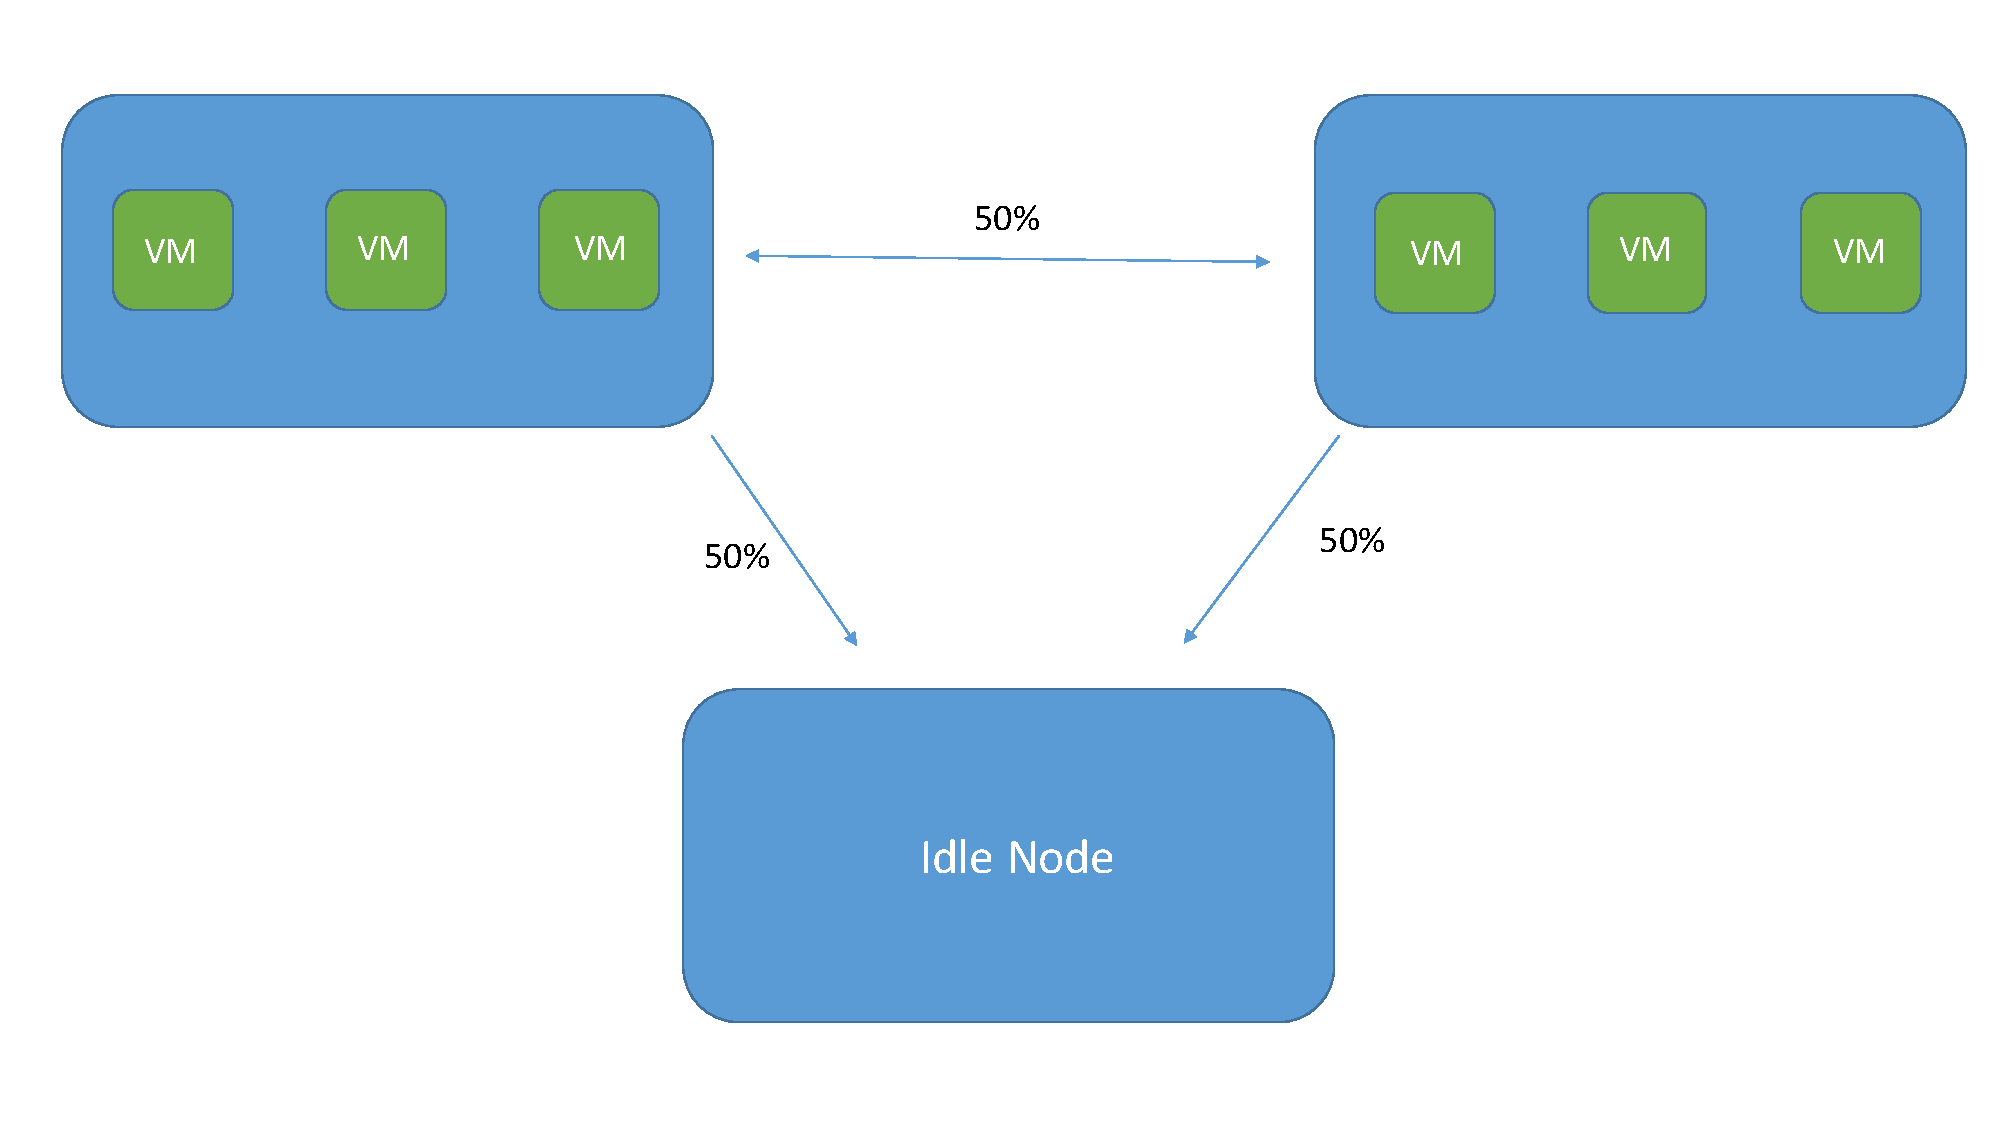
\includegraphics[scale=0.4]{images/homogeneous_workload_disparity.pdf} 
      \caption{A cluster with identical nodes running a heterogeneous workload.}
      \label{fig:workload_disparity}
    \end{figure}

    \subsubsection{Nodes with Tier Size Disparities}

    A cluster containing nodes with a tier size disparity are susceptible to a
    skew in node fullness, even if the workload on each node is identical. This
    can be illustrated via Figure \ref{fig:tier_size_disparity} where we have a
    3-node heterogeneous cluster with 2 high-end nodes and a single weak node.
    Suppose these high-end nodes have 500GB of SSD tier and 6TB of HDD tier and
    the single weak node has only 128GB of SSD tier and 1TB of HDD tier. If 3
    simultaneous workloads were to generate data such that the working sets of
    the workloads are 50\% of the local SSD tier, the weaker node is at a
    significant disadvantage. Given the current ADSF replica selection
    algorithm, we can expect 500GB of replica traffic to flood the weak node
    and fill up its SSD tier well before the workload is finished. This results
    in an inability for the workload on the smaller node to place its primary
    replicas locally and forces the workload to rely on remote CVMs, increasing
    latency. An adaptive replica placement heuristic would mitigate this issue
    by taking disk usages into consideration during the placement of secondary
    replicas and biasing placement of secondary replicas on the nodes with more
    free capacity.

    \begin{figure}[h]
      \centering
      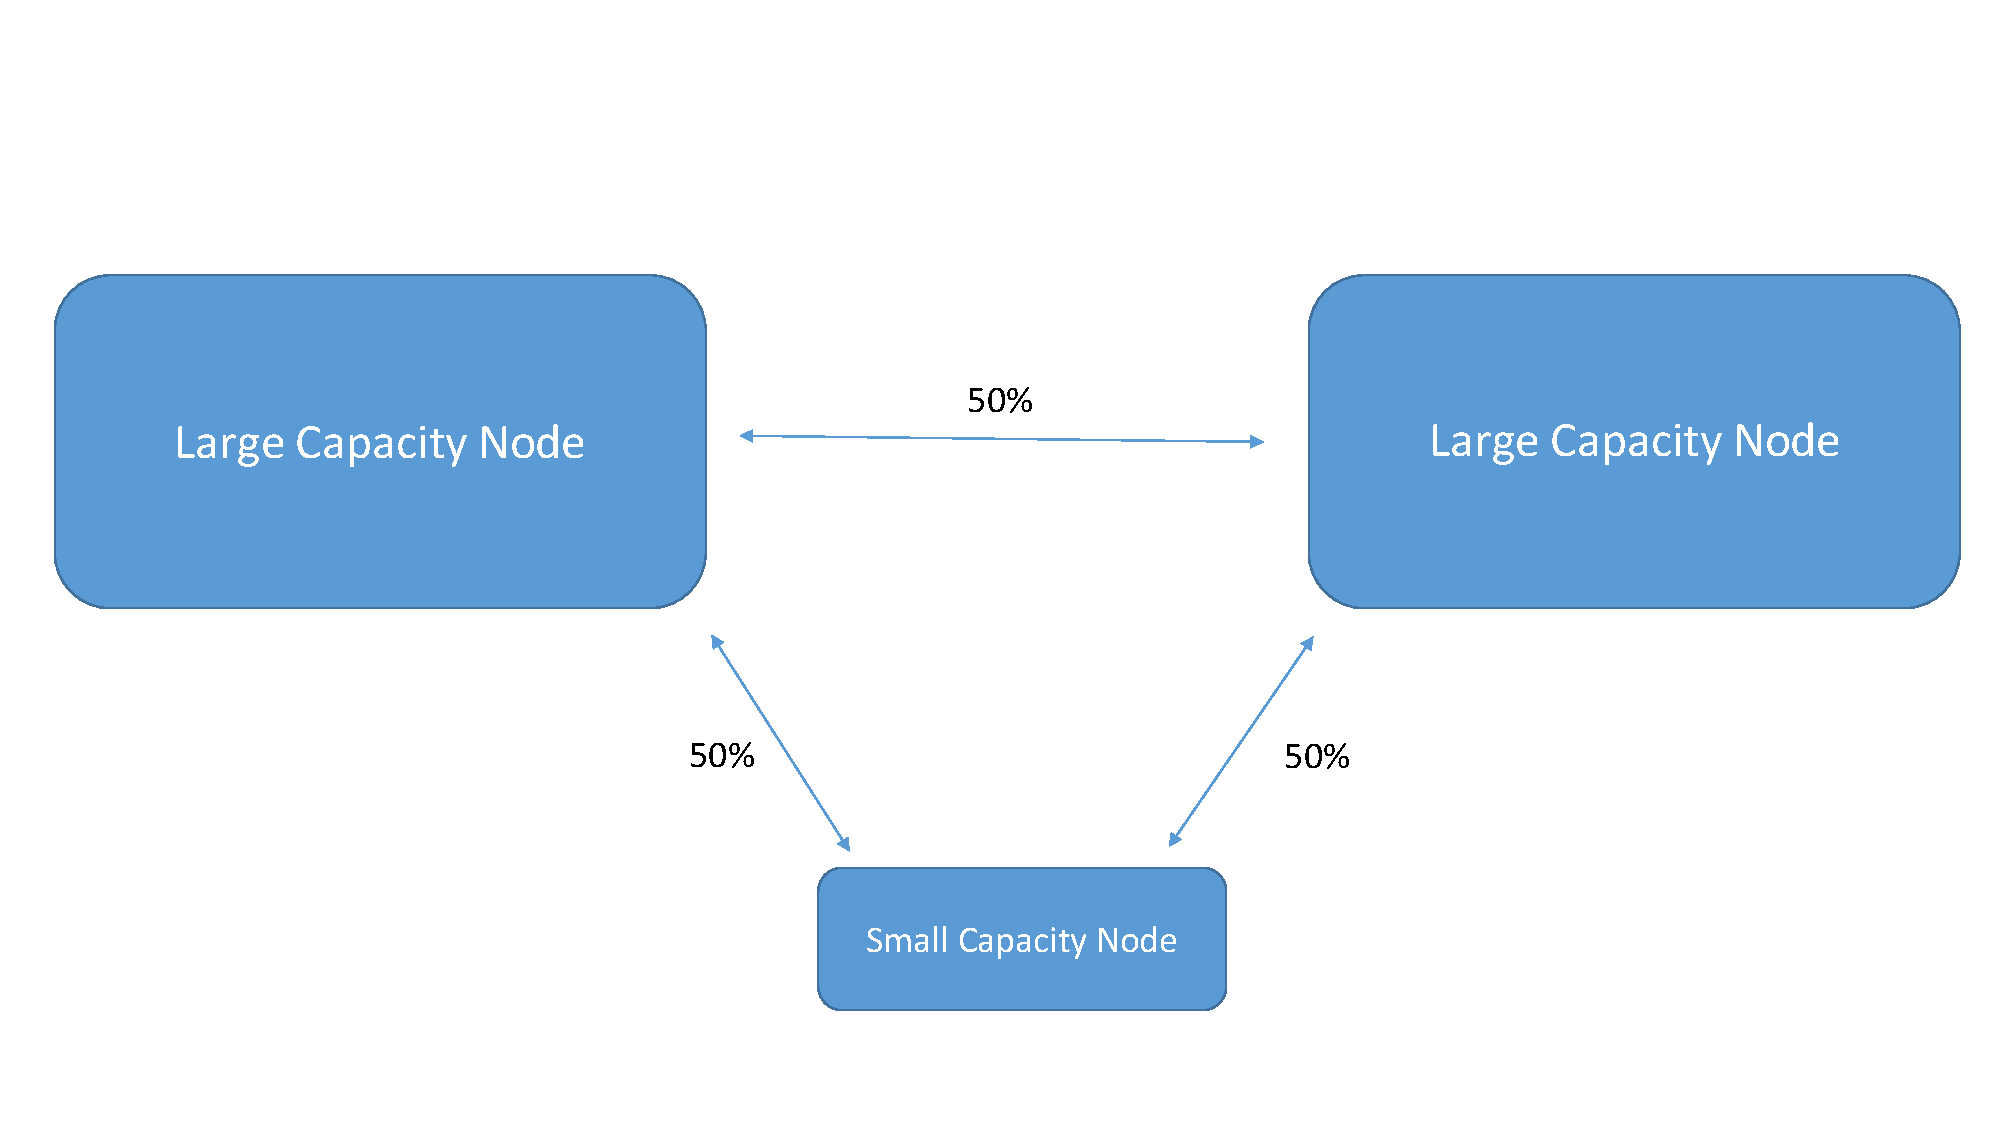
\includegraphics[scale=0.4]{images/homogeneous_tier_disparity.pdf} 
      \caption{A cluster with nodes of varying resource capacity.}
      \label{fig:tier_size_disparity}
    \end{figure}

  \subsection{Acropolis Base System}

  ADSF is facilitated by a clustering of controller virtual machines (CVMs)
  which reside, one per node, on each server in the cluster. The CVM presents
  via NFS (for VMWare's ESXi \cite{esxi2008}), SMB (for Microsoft's Hyper-V
  \cite{hyperv2009}), or
  iSCSI (for Nutanix's AHV \cite{bible}) an interface to each hypervisor that they
  reside on. For example, the interface provided by the CVMs to VMware's ESXi
  hypervisor will be interfaced with as a datastore. The virtual machines'
  virtual disk files will reside on the Nutanix datastore and be accessed via
  NFS through the CVM sharing a host with the user VM. Within the CVM exists an
  ecosystem of process that make up the ADSF. This work is scoped specifically
  to the I/O manager process, Stargate.


  \subsection{Stargate}

  The Stargate process is responsible for all data management and I/O
  operations. The NFS/SMB/iSCSI interface presented to the hypervisor is also
  presented by Stargate. All file allocations and data replica placement
  decisions are made by this process.

  As the Stargate process facilitates writes to physical disks, it gathers
  statistics for each disk such as the number of operations currently in flight
  on the disk (queue length), how much data in bytes currently resides on the
  disk, and average time to complete an operation on the disk. These statistics
  are only gathered on the local disks; however, they are then stored in a
  distributed database provided by another ADSF service, Arithmos, along with
  the statistics gathered by every other Stargate in the cluster. These disk
  statistics stored in the database and are pulled periodically and are then
  used to make decisions on data placement when performing writes.

    \subsubsection{The Extent Store}

    The Extent Store is a sub-component of Stargate that serves as the
    persistent bulk storage. Data stored within the Extent Store are referred
    to as extent groups (also referred to as egroups), or 4MB pieces of
    physically contiguous data. These extent groups are replicated a number of
    times dependent on the cluster replication factor and each replica is
    placed on a different CVM except for a single replica that resides on the
    local node. The current replica selection algorithm will be explained in
    further detail in the "Replica Selection" section.

    \subsubsection{Storage Tiering and Data Replication}

    Data in the system is physically stored on disks of varying type. Within a
    given cluster, one can find NVMe, PCIe SSD, SATA SSD, and HDD drive types.
    These disks are separated out into groupings of similar drive types
    referred to as storage tiers. Extent groups and their replicas are created
    on a particular storage tier, but may be migrated between tiers depending
    on data access patterns.

    Data replicas for each extent group are written on separate fault domains
    on the same tier to ensure that in the event a failure occurs and a
    replica becomes unavailable, that piece of data can still be accessed. An
    example of a fault domain can be a node (single CVM) or a block (a rackable
    unit of hardware containing multiple nodes). 

    \subsubsection{Replica Selection}

    When a Stargate write operation wants to select disks for data placement
    upon entrance into the Extent Store, it is done on a per-tier basis. The
    interface for a replica selection function call, DetermineNewReplicas,
    takes the following arguments:

    \begin{center}
      \begin{tabular}{ | p{0.4\linewidth} | p{0.6\linewidth} | }
        \hline
        \textbf{Argument Name} & \textbf{Description} \\ \hline
        \verb|replica_vec| & A std::vector that is populated with the selected
                             disk IDs. The number of selections made is the
                             size of this vector. \\ \hline

        \verb|storage_tier| & The name of the storage tier (set of disks) to
                              select for data placement. \\ \hline
 
        \verb|storage_pool_vec| & The collection of all disks in the cluster.  \\ \hline

        \verb|preferred_node_vec| & Nodes we prefer to choose disks from. This
                                    means we will consider disks from these
                                    nodes first and only consider other disks
                                    if the ones belonging to these nodes are
                                    not suitable. \\ \hline

        \verb|predicate_func| & A function that accepts a disk ID and returns a
                                boolean. If this function evaluates to false
                                for any disk, it is not considered for
                                selection. \\ \hline

        \verb|exclude_replica_vec| & Disk IDs that will be excluded from
                                     selection. \\ \hline

        \verb|exclude_node_vec| & Node IDs whose disks will be excluded from
                                  selection. \\ \hline

        \verb|exclude_rackable_unit_vec| & Rack IDs whose disks will be
                                           excluded from selection. \\ \hline

        \hline
      \end{tabular}
    \end{center}

    Upon calling DetermineNewReplicas, we first attempt to select replicas from
    the preferred nodes. This involves finding the set of disks that belong to
    each node on the specified tier, shuffling the disks, and sequentially
    evaluating each disk until a suitable one is found (the evaluation step).
    If a suitable disk is not found on a preferred node, all other disks
    belonging to the specified tier are shuffled and considered sequentially
    until enough disks are found to satisfy the requirement set by replica\_vec.

    A suitable disk is one that:

    \begin{enumerate}
      \item Contains enough space to accept new data. This is less than 95\% by
            default for Nutanix clusters.  \item Returns "true" when evaluated by the
            predicate\_func.
      \item Is not included in the exclude\_replic\_vec, exclude\_node\_vec,
            and exclude\_rackable\_unit\_vec.
    \end{enumerate}

    If a disk does not meet the criteria above, we simply continue searching
    the shuffled set of disks belonging to the specified tier. If a disk is
    found to be suitable, we must add the disk to the replic\_vec and add the
    node that the disk belongs to in the exclude\_nod\_vec. This prevents us
    from considering other disks on that node to maintain a node fault
    tolerance guaranteed by the cluster's replication factor.

%%%%%%%%%%%%%%%%%%%%%%%%%%%%%%%%%%%%%%%%%%%%%%%%%%%%%%%%%%%%%%%%%%%%%%%%%%%%%%%

\section{Prior Work}

Xie et. al. showed that data placement schemes based on the computing
capacities of nodes in the Hadoop Distributed File System (HDFS) significantly
improved workload performance \cite{hdfs2008}. These computing capacities are
determined for each node in the cluster by profiling a target application
leveraging the
HDFS. Their MapReduced wordcount and grep results showed up to a 33.1%
reduction in response time. Similarly, Perez et. al. applied adaptive data
placement features to the Expand parallel file system based on available free
space \cite{perez2003}. Though effective in their given contexts, the main drawback to this
work is that it assumes the specific application is working without
interference and does not account for other workloads on the system.

One adaptive data placement approach that can account for other workloads on
the system was introduced by Jin et. al. in their work on ADAPT
\cite{adapt2012}. The work
predicts how failure-prone a node in a MapReduce cluster is and advises their
availability-aware data placement algorithm to avoid those nodes. This proves
useful for performance by avoiding faulty nodes that could fail mid-task and
cause data transfers and re-calculation of data.

Work by Suresh et. al. approaches adaptive replica selection in much the same
way proposed in this paper, though their work was mainly focused on decreasing
tail latencies for Cassandra reads \cite{suresh2015}. Their load balancing algorithm, C3,
incorporates the concept of a value calculated from request feedback from their
servers that allows for decisions to be made on server selection. In addition
to the ranking function in C3, they implemented a distributed rate control
mechanism to prevent scenarios where many individual clients can bombard a
single highly desirable server with requests. Many of the same problems that
the work in this proposal seeks to remedy are also addressed by the C3
algorithm; however, given the Nutanix file system's architecture, some C3
solutions are not feasible.

The C3 algorithm takes into account the request queue length of certain servers
similar to the way I will use disk queue lengths. In addition Suresh et. al.
factor in the service latencies of each server so that they may consider a
different ideal queue length for each server. With this approach, longer
service times will warrant a lower queue length and vice versa. This is
beneficial for scenarios where there are multiple underlying storage
technologies such as NVMe drives, SSDs, and HDDs under consideration, but the
Nutanix file system's architecture does not allow for multiple replicas to span
storage tiers. This forces the ideal queue lengths for each selection pool to
be the same. Therefore, my work does not incorporate service latencies in the
fitness value calculations.

Herding of requests to a single highly suitable server is a problem that arises
in any replica ranking algorithm. C3 mitigates this issue by rate limiting
client requests to each server via a decentralized calculation using a
configured time interval and local sending rate information. I've opted to use
a simpler probabilistic spreading of client requests via selecting remote nodes
using a weighted random selection tied to the calculated fitness values.

%%%%%%%%%%%%%%%%%%%%%%%%%%%%%%%%%%%%%%%%%%%%%%%%%%%%%%%%%%%%%%%%%%%%%%%%%%%%%%%

\section{Implementation}

  \subsection{Stargate Disk Stats Collection}

  Prior to this work, Stargate's periodic disk stats collection was limited to
  caching solely disk usage stats for all disks in the cluster.  This has been
  expanded to now include disk performance stats for use in disk fitness
  values.

  Stargate maintains a mapping, henceforth referred to as the $disk\_map\_$,
  from cluster disk ID to a disk state structure. The $disk\_map\_$'s state
  structure contains disk usage and performance information that has been
  published to Arithmos by other Stargates in the cluster. Upon gathering fresh
  stats from Arithmos, the information is used to create a disk fitness value
  for each disk in the cluster.

  \subsection{Fitness Values and Functions}

  To calculate a value to represent the desirability of a disk for replica
  placement, we'll use a function, $f_{fitness}$ that takes as its argument
  disk stats and returns a positive number we will call a fitness value. A low
  fitness value indicates a poor placement candidacy for a disk and a high
  fitness value will indicate a highly desirable disk for replica placement. In
  this thesis, I evaluate two fitness functions that are comprised of terms
  that utilize a disk's average queue length over some stretch of time,
  $t_{q}$, and a disk's percentage utilization, $t_{u}$.

  \begin{equation}
    t_{q} = 1 - \frac{q}{q_{ceil}}
  \end{equation}

  $q_{ceiling}$ is defined as the maximum observed queue length such that
  beyond this value, $t_{q}$ does not contribute to the fitness
  value. This ensures that as the queue length grows, $t_{q}$
  approaches zero. 

  \begin{equation}
    t_{u} = \frac{1}{a^{u}}
  \end{equation}

  $u$ is the disk utilization percentage and $a$ is an aggression variable used
  to control the exponential decay of $t_{u}$. The larger $a$ is, the
  more aggressively $t_{u}$ will decay as $u$ increases. An
  aggressive decay results in more preference given to less utilized disks when
  compared with disks that are slightly more utilized.

  These terms are used in two different fitness functions evaluated in this
  thesis:

  \begin{equation}
    f_{add} = t_{u} + t_{q}
  \end{equation}

  \begin{equation}
    f_{mult} = t_{u}t_{q}
  \end{equation}


  \subsection{Weighted Random Selection Algorithms}

  After a weight is calculated for a disk in the cluster that will store a
  replica, the WeightedVector class' Sample() calls will perform a weighted
  random selection on the set of potential candidate disks. To determine the
  best method of weighted random selection for Stargate's WeightedVector class,
  an exploration of various weighted random selection algorithms was necessary.
  Since the file system only supports replication factors of 2 or 3, the
  investigation was limited to algorithms that allow for a weighted $N$ choose
  $Y$, where $Y$ is the data replication factor.

  This section provides an overview of the algorithms investigated via
  simulations to compare each algorithm at different orders of magnitude.

    \subsubsection{Scalability Simulation Methodology}
     To test the scalability of the weighted random selection algorithms
     evaluated in the next section, a single-threaded Python \cite{python}
     script was written to to evaluate the change in run time as sample sets
     increase. Each algorithm's time to select is calculated for each of a
     fixed number of iterations for multiple sample sets. pseudo-code for the
     simulations can be written as follows:

     \begin{verbatim}
     for each selection_algorithm in algorithm_list:
         run_time_values = empty_list()
         for each sample_set_size in all_sample_set_sizes:
             sample_set = generate_sample_set(sample_set_size)
             all_elapsed_times = empty_list()
             for each iteration:
                 start_time = time.now()
                 selection_algorithm(sample_set)
                 elapsed_time = time.now() - start_time
                 all_elapsed_times.append(elapsed_time)
             calculate_avg_elapsed_time(all_elapsed_times)
             calculate_std_error(all_elapsed_times)
     \end{verbatim}
        
    Object weights are constant throughout the simulation, so selection schemes
    that require some amount of preprocessing (such as the top T\% calculation
    for truncation selection) are performing their preprocessing steps for each
    selection. This gives information about the worst-case behavior for each
    algorithm in comparison with others'.

    \subsubsection{Herding Behavior Evaluation Methodology}
    Herding behaviors can be seen in some weighted random selection
    algorithms when the weights of a subset of objects in the sampling pool
    cause a disproportionate amount of selections to target those objects. In
    the case of replica disk selections in a Nutanix cluster, this can cause
    too many operations to target an especially suitable disk, resulting in
    poor performance. We can simulate an exaggerated scenario in which the
    susceptibility to herding behavior can be observed by having a single
    object with a weight that is multiple orders of magnitude heavier than the
    next highest object in the sampling set. It is also necessary to observe
    any herding behavior for a sampling set with low weight skew. This section
    describes the simulation methodology for each.

    High-skew sampling sets of 11 objects were generated such that the array
    index of the first 10 objects was assigned as the object weight, and the
    last object was given a weight of 1000. This creates an extremely large
    skew in weights and makes the high-weight object a target for herding
    behavior. Given this sampling set, weighted random selections were
    performed and a histogram was kept that tracked the number of selections
    for each object. $10^3$, $10^4$, and $10^5$ iterations were performed to observe any
    changes in herding behavior at larger time scales. In addition to the
    high-skew sampling sets, low-skew sets of 100 objects were also simulated.
    These low-skew sets were identical to the high-skew sets, except there was
    not a single object with an exaggerated weight of 1000. All element weights
    were their array indices.

    \subsubsection{Stochastic Universal Sampling (SUS) Simulations}
    SUS is another sampling technique first introduced by Baker in 1987
    \cite{baker1987}.
    The algorithm can be understood as follows: On a standard roulette wheel
    there's a single pointer that indicates the winner. The roulette wheel's
    "bins" can all be the same size which would indicate a uniform probability
    of selecting any bin and could also be unevenly sized which would indicate
    a weighted probability. SUS uses this same concept except allows for N
    evenly spaced pointers corresponding to the selection of N items. Key
    things to note are that the set, or "bins" in my roulette analogy, must be
    shuffled prior to selection. Also, there is a minimum spacing allowed for
    the pointers to prevent selection of the same bin.

    \begin{figure}[h]
      \centering
      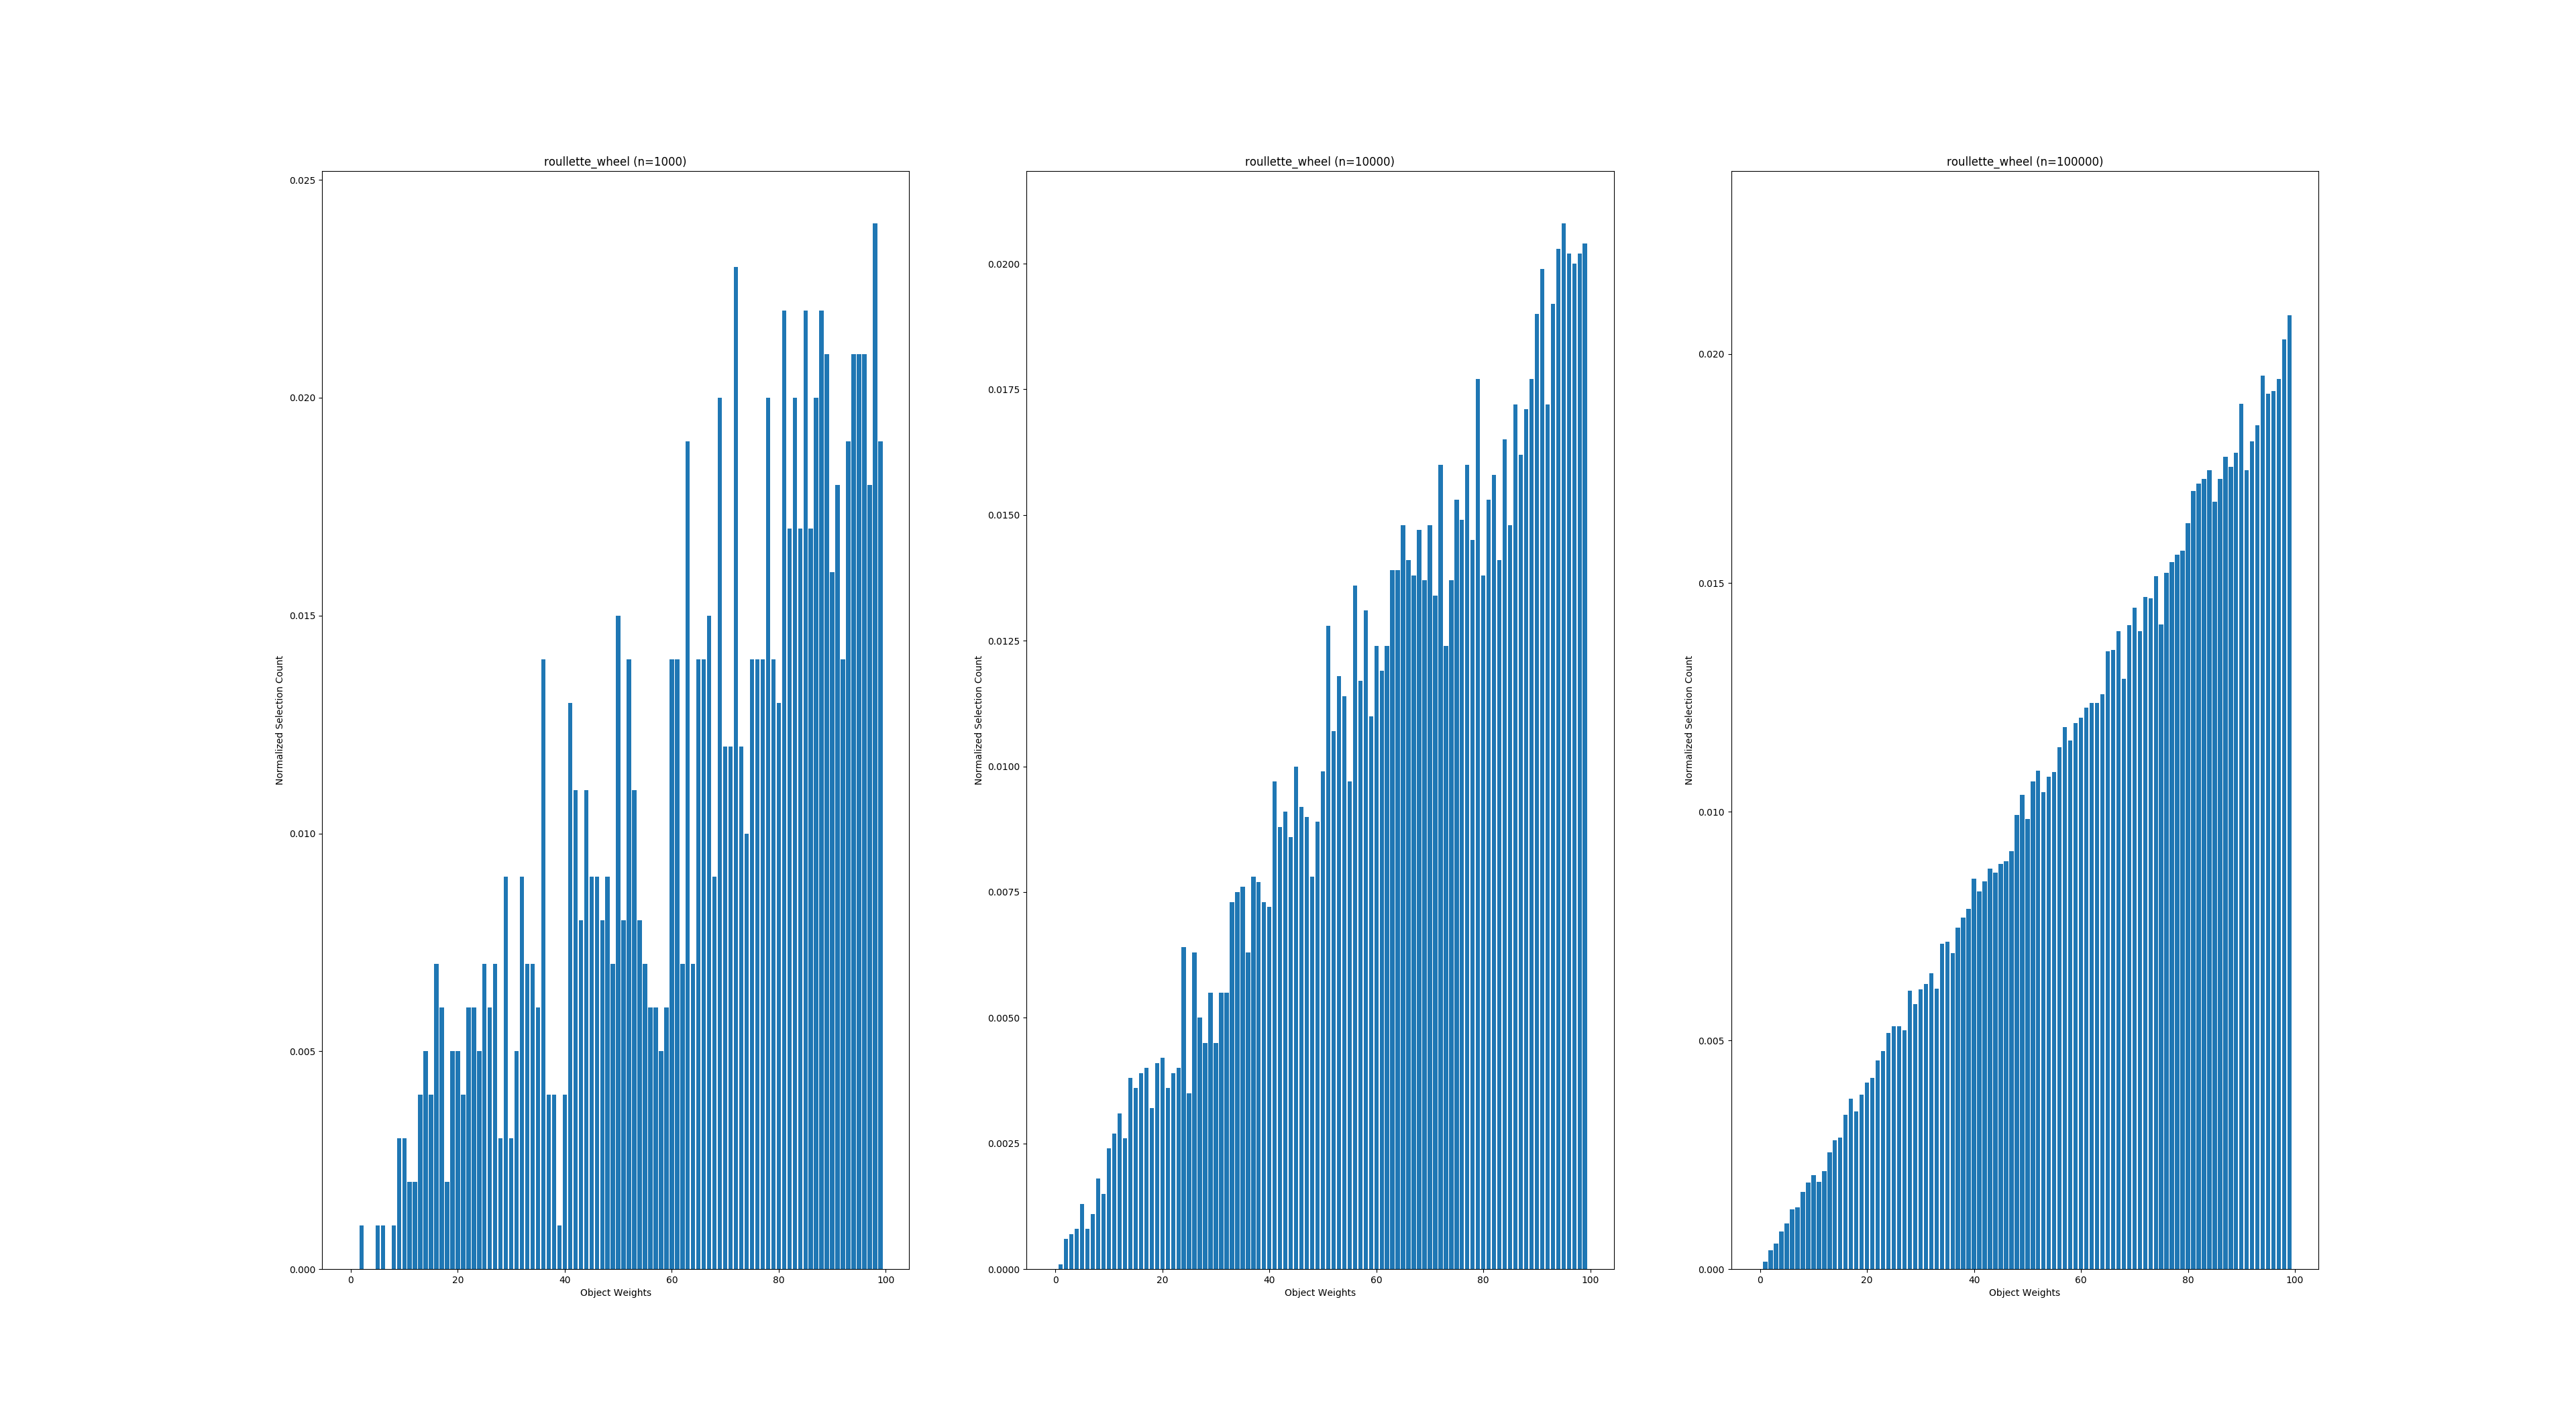
\includegraphics[scale=0.30]{images/herding_roullette.png} 
      \caption{Histograms generated by simulation of Stochastic Universal
               Sampling using sample sizes of 1e3, 1e4, and 1e5. Object weights
               for the histograms are in the range [1,100].}
      \label{fig:herding_roullette}
    \end{figure}

    \begin{figure}[h]
      \centering
      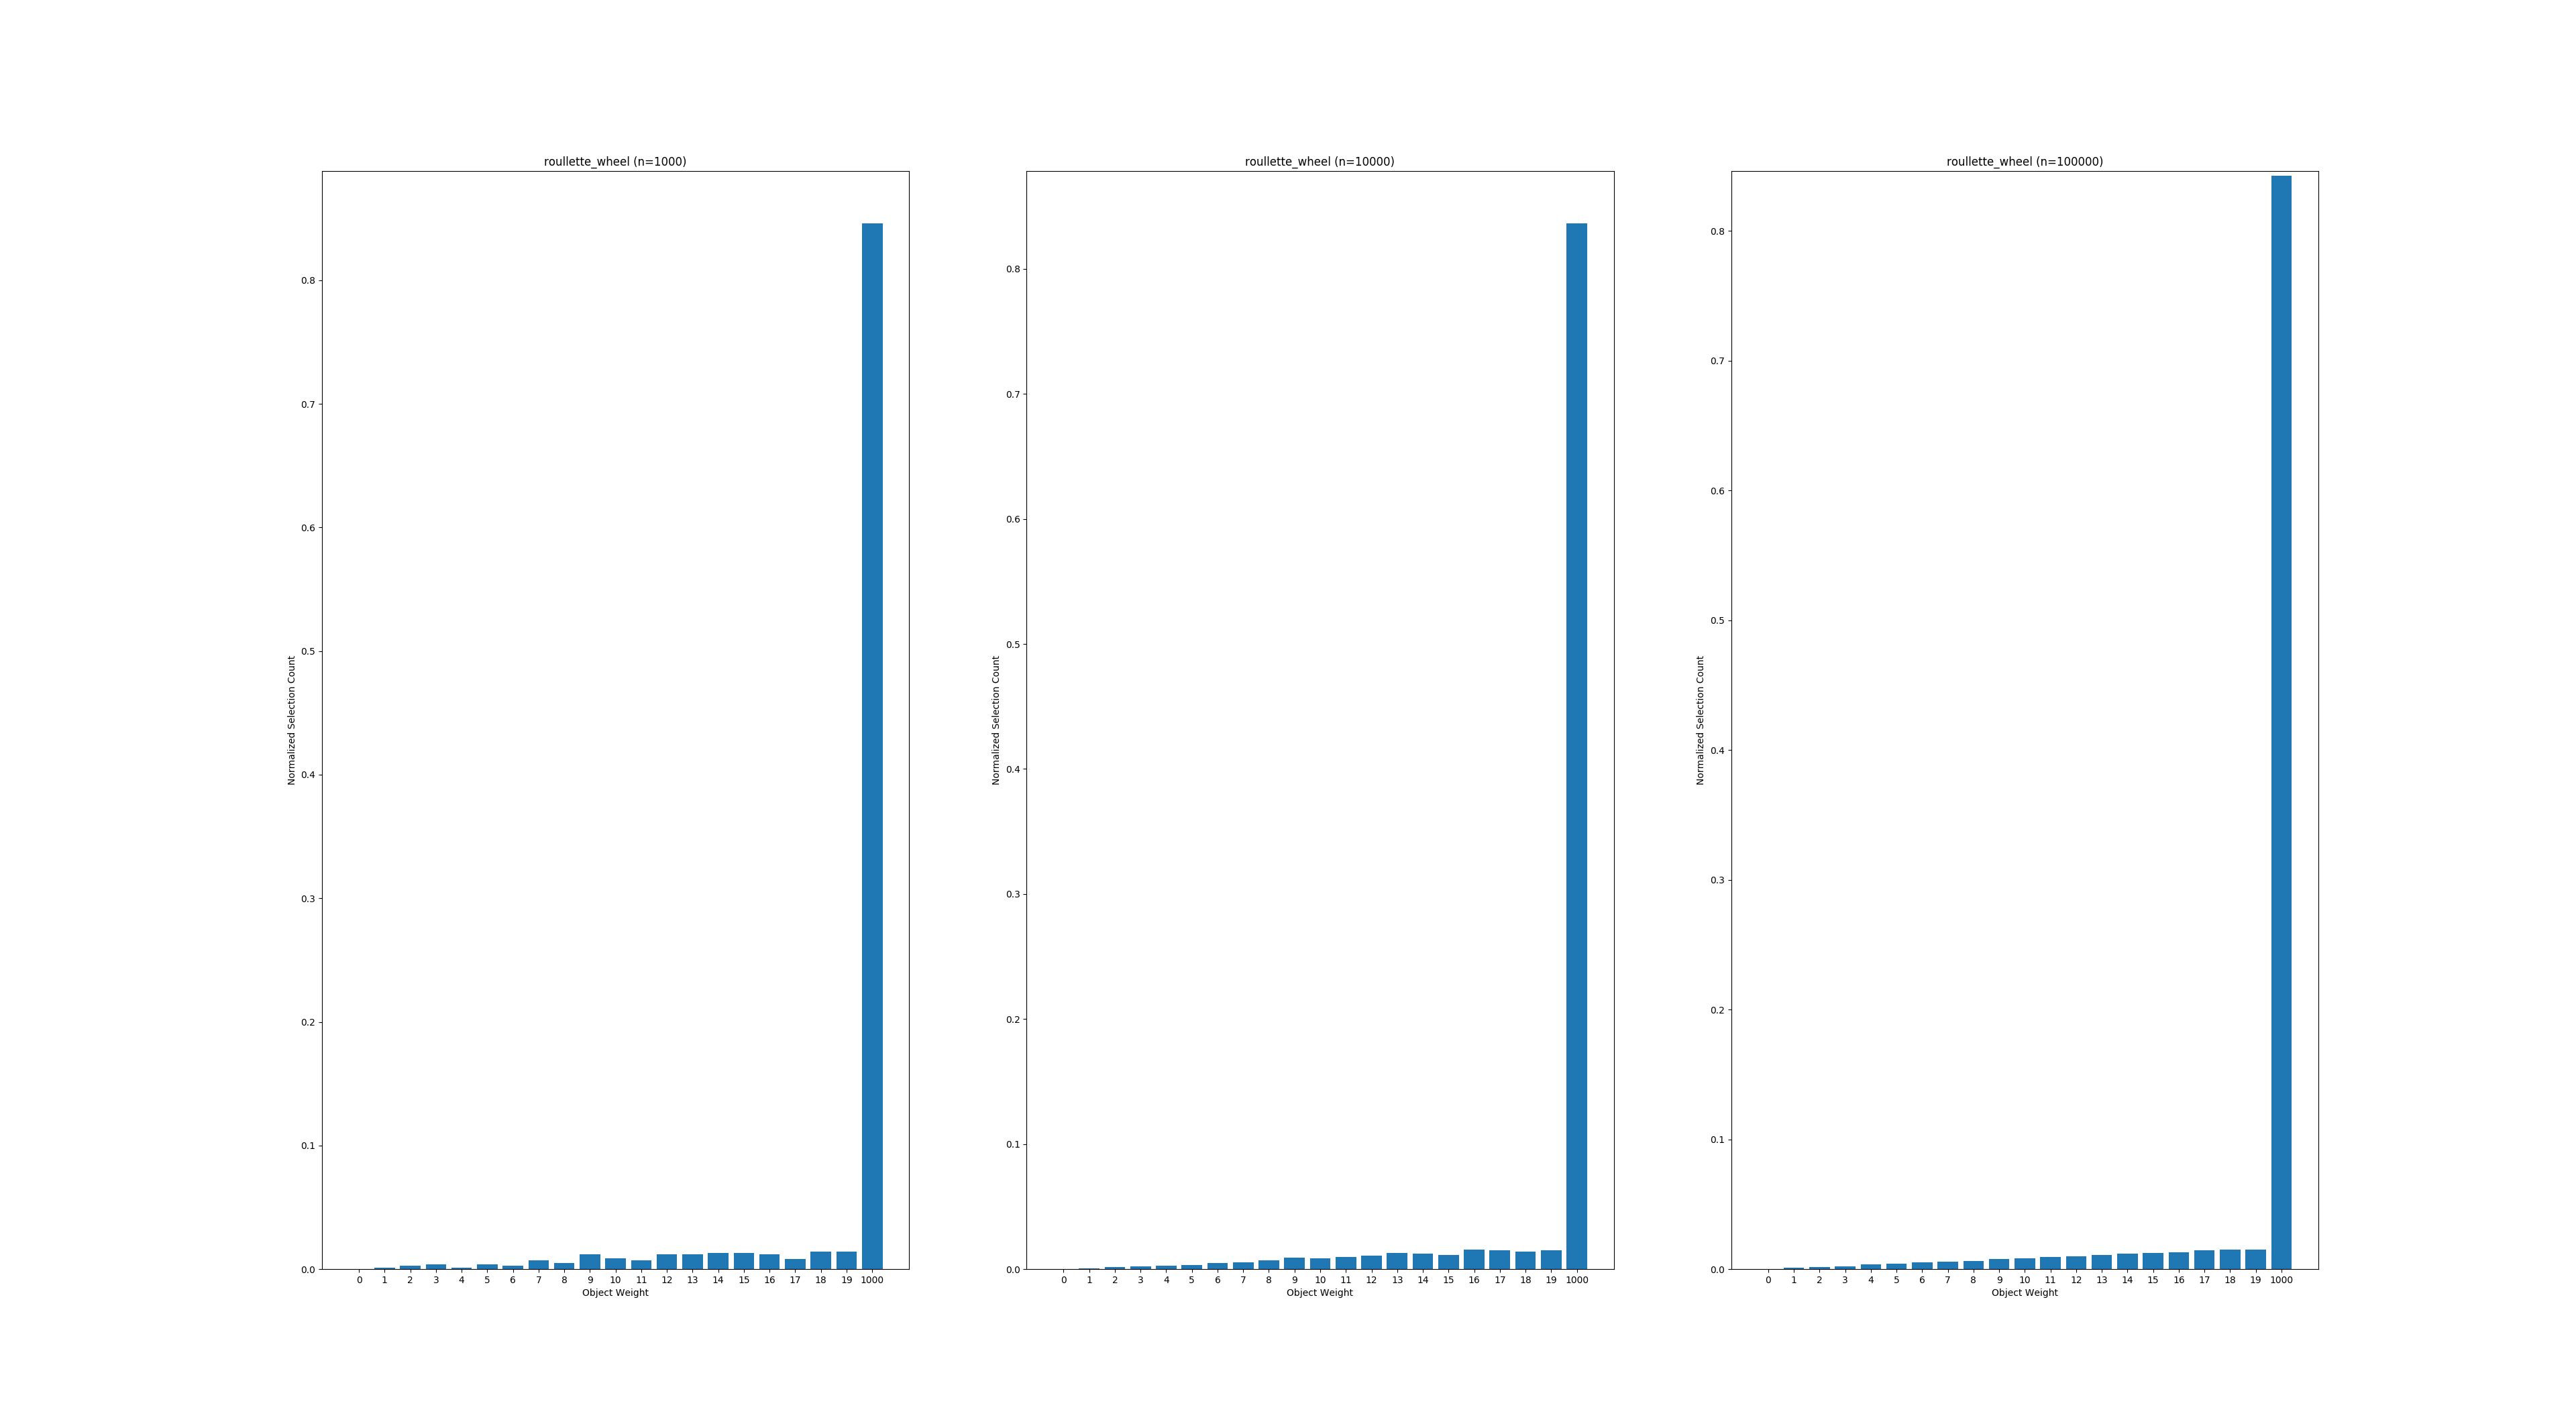
\includegraphics[scale=0.30]{images/pathological_roullette.png} 
      \caption{Histograms generated by simulation of Stochastic Universal
               Sampling using sample sizes of 1e3, 1e4, and 1e5. Object weights
               are in the range [0,9] with a single outlier of weight 1000 to
               illustrate the effect of herding behavior.}
      \label{fig:pathological_roullette}
    \end{figure}

    Figure \ref{fig:herding_roullette} shows the evolution of the
    distribution of selection frequencies for SUS as the number of samples
    increases. We can see that the selection frequency is proportional to the
    object weight. This can prove problematic for outlier objects with weights
    that are much larger than the other objects in the set as shown in Figure
    \ref{fig:pathological_roullette}. We can see that the high weight object's
    selection frequency eclipses all other objects in the selection pool which
    can lead to extreme herding behaviors.

    \subsubsection{Tructation Selection Simulations}
    Truncation selection \cite{truncation1973} does not consider any objects
    for selection below some threshold, $T$. In figure
    \ref{fig:herding_truncation}, only the top 10\% of objects ranked by weight
    are considered for selection. Within this subset, weight has no meaning so
    there is a uniform distribution of selections. However, this may not be
    suitable for use cases where all objects must be candidates for selection.
    Depending on the threshold chosen, this algorithm can be resistant to
    herding behavior as shown in Figure \ref{fig:pathological_truncation}. 

    \begin{figure}[h]
      \centering
      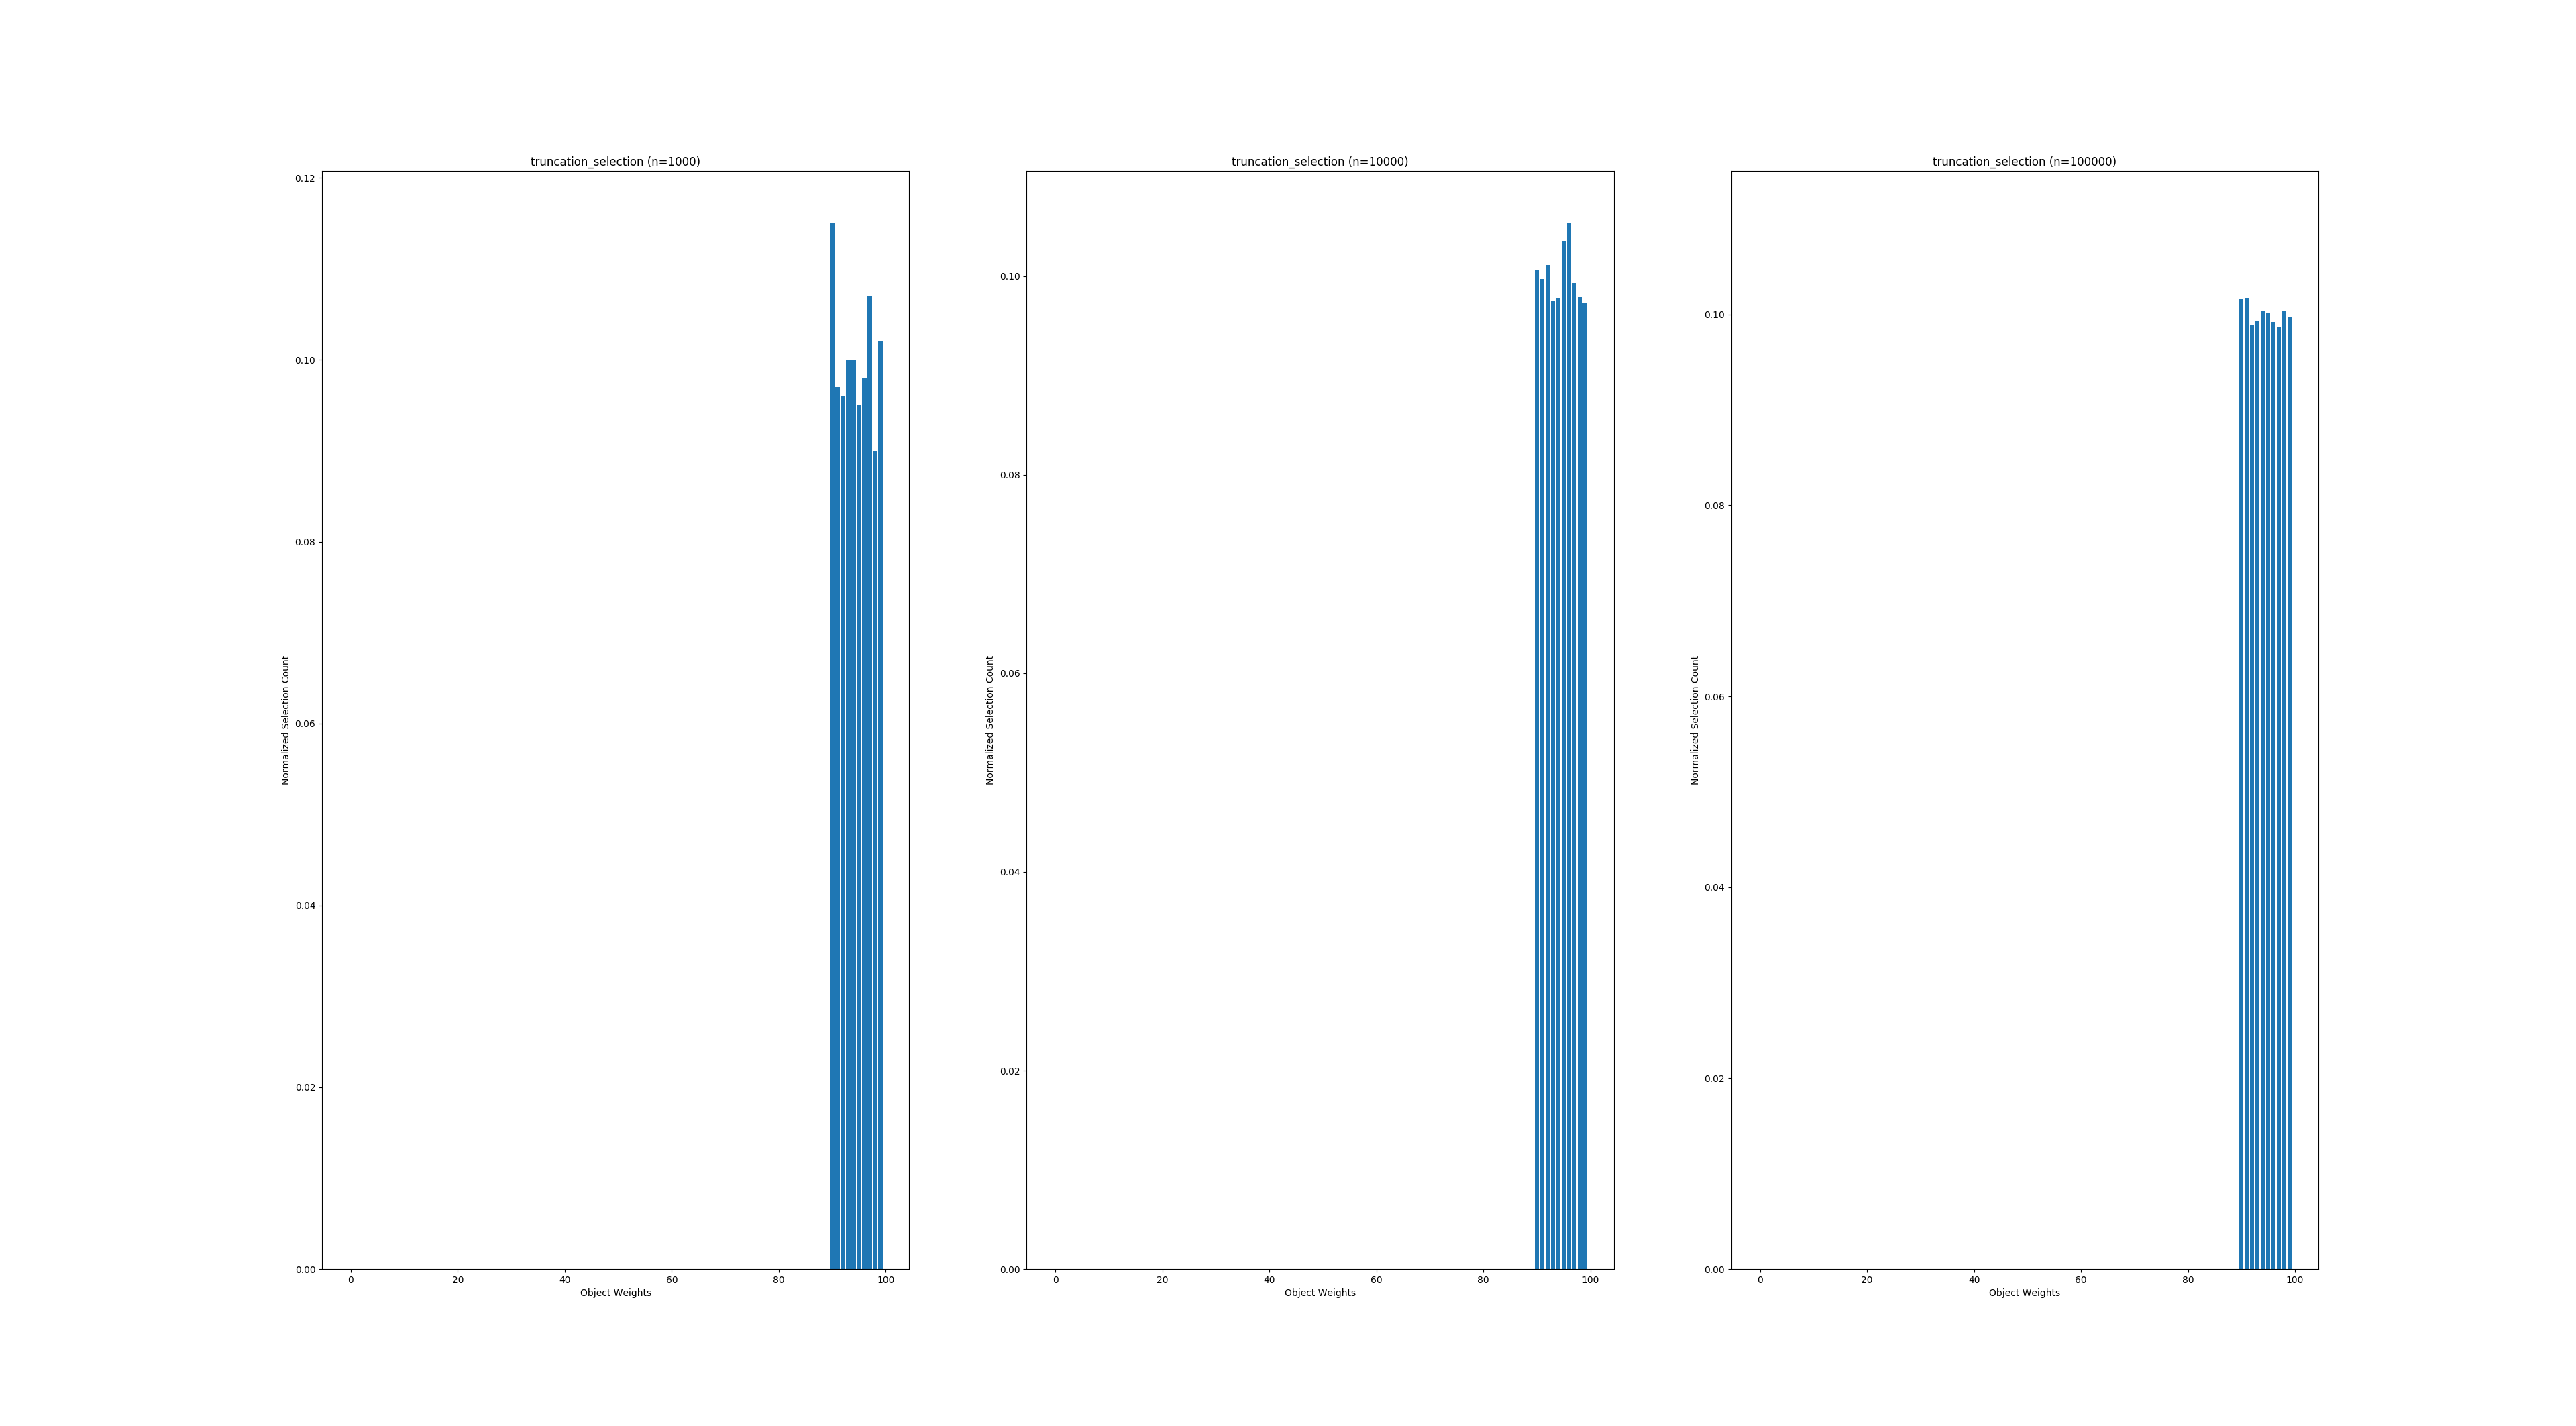
\includegraphics[scale=0.30]{images/herding_truncation.png} 
      \caption{Histograms generated by simulation of truncation selection
               using sample sizes of 1e3, 1e4, and 1e5. Object weights
               for the histograms are in the range [1,100].}
      \label{fig:herding_truncation}
    \end{figure}

    \begin{figure}[h]
      \centering
      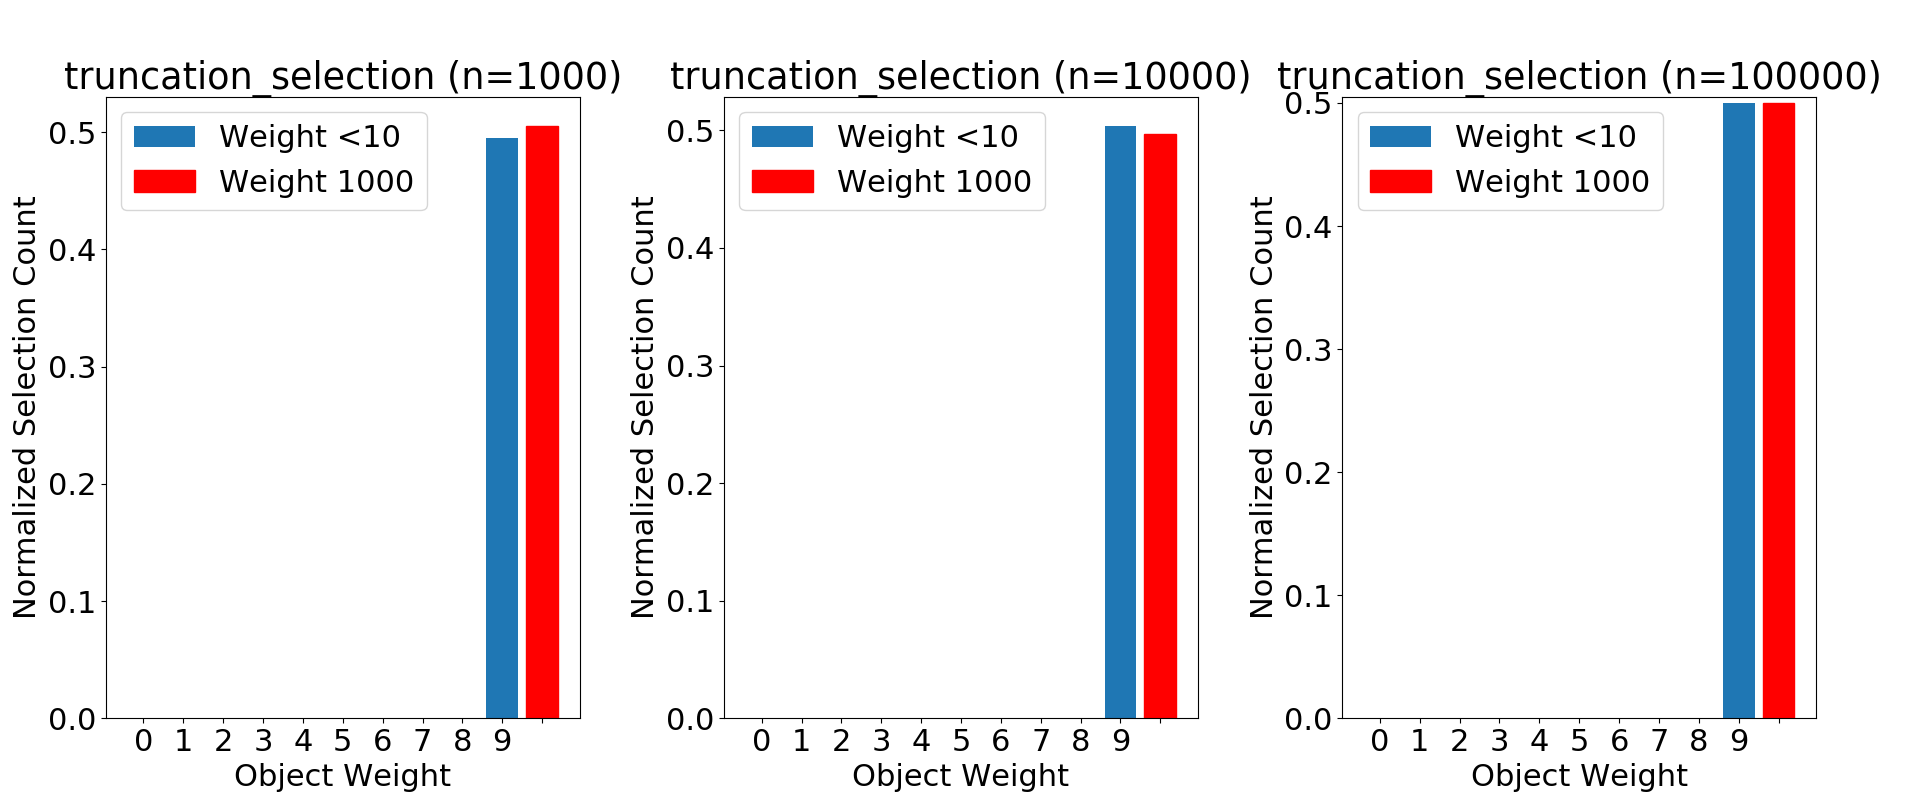
\includegraphics[scale=0.30]{images/pathological_truncation.png} 
      \caption{Histograms generated by simulation of truncation selection
               using sample sizes of 1e3, 1e4, and 1e5. Object weights are in
               the range [0,9] with a single outlier of weight 1000 to
               illustrate the effect of herding behavior.}
      \label{fig:pathological_truncation}
    \end{figure}

    \subsubsection{Two-choice Sampling Simulations}
    Two-choice sampling \cite{2choice}, has proven to be extremely resilient to
    herding behavior as shown in Figure \ref{fig:pathological_two_choice} and
    selection frequencies for all objects are influenced by object weights in a
    way similar to SUS. While an object with a higher weight is more likely to
    be selected, it is not selected with a probability proportional to its
    fitness value. This makes the algorithm resistant to any herding behaviors,
    but will not be a good candidate if we desire the WeightedVector to select
    objects with probability proportional to its weight.

    \begin{figure}[h]
      \centering
      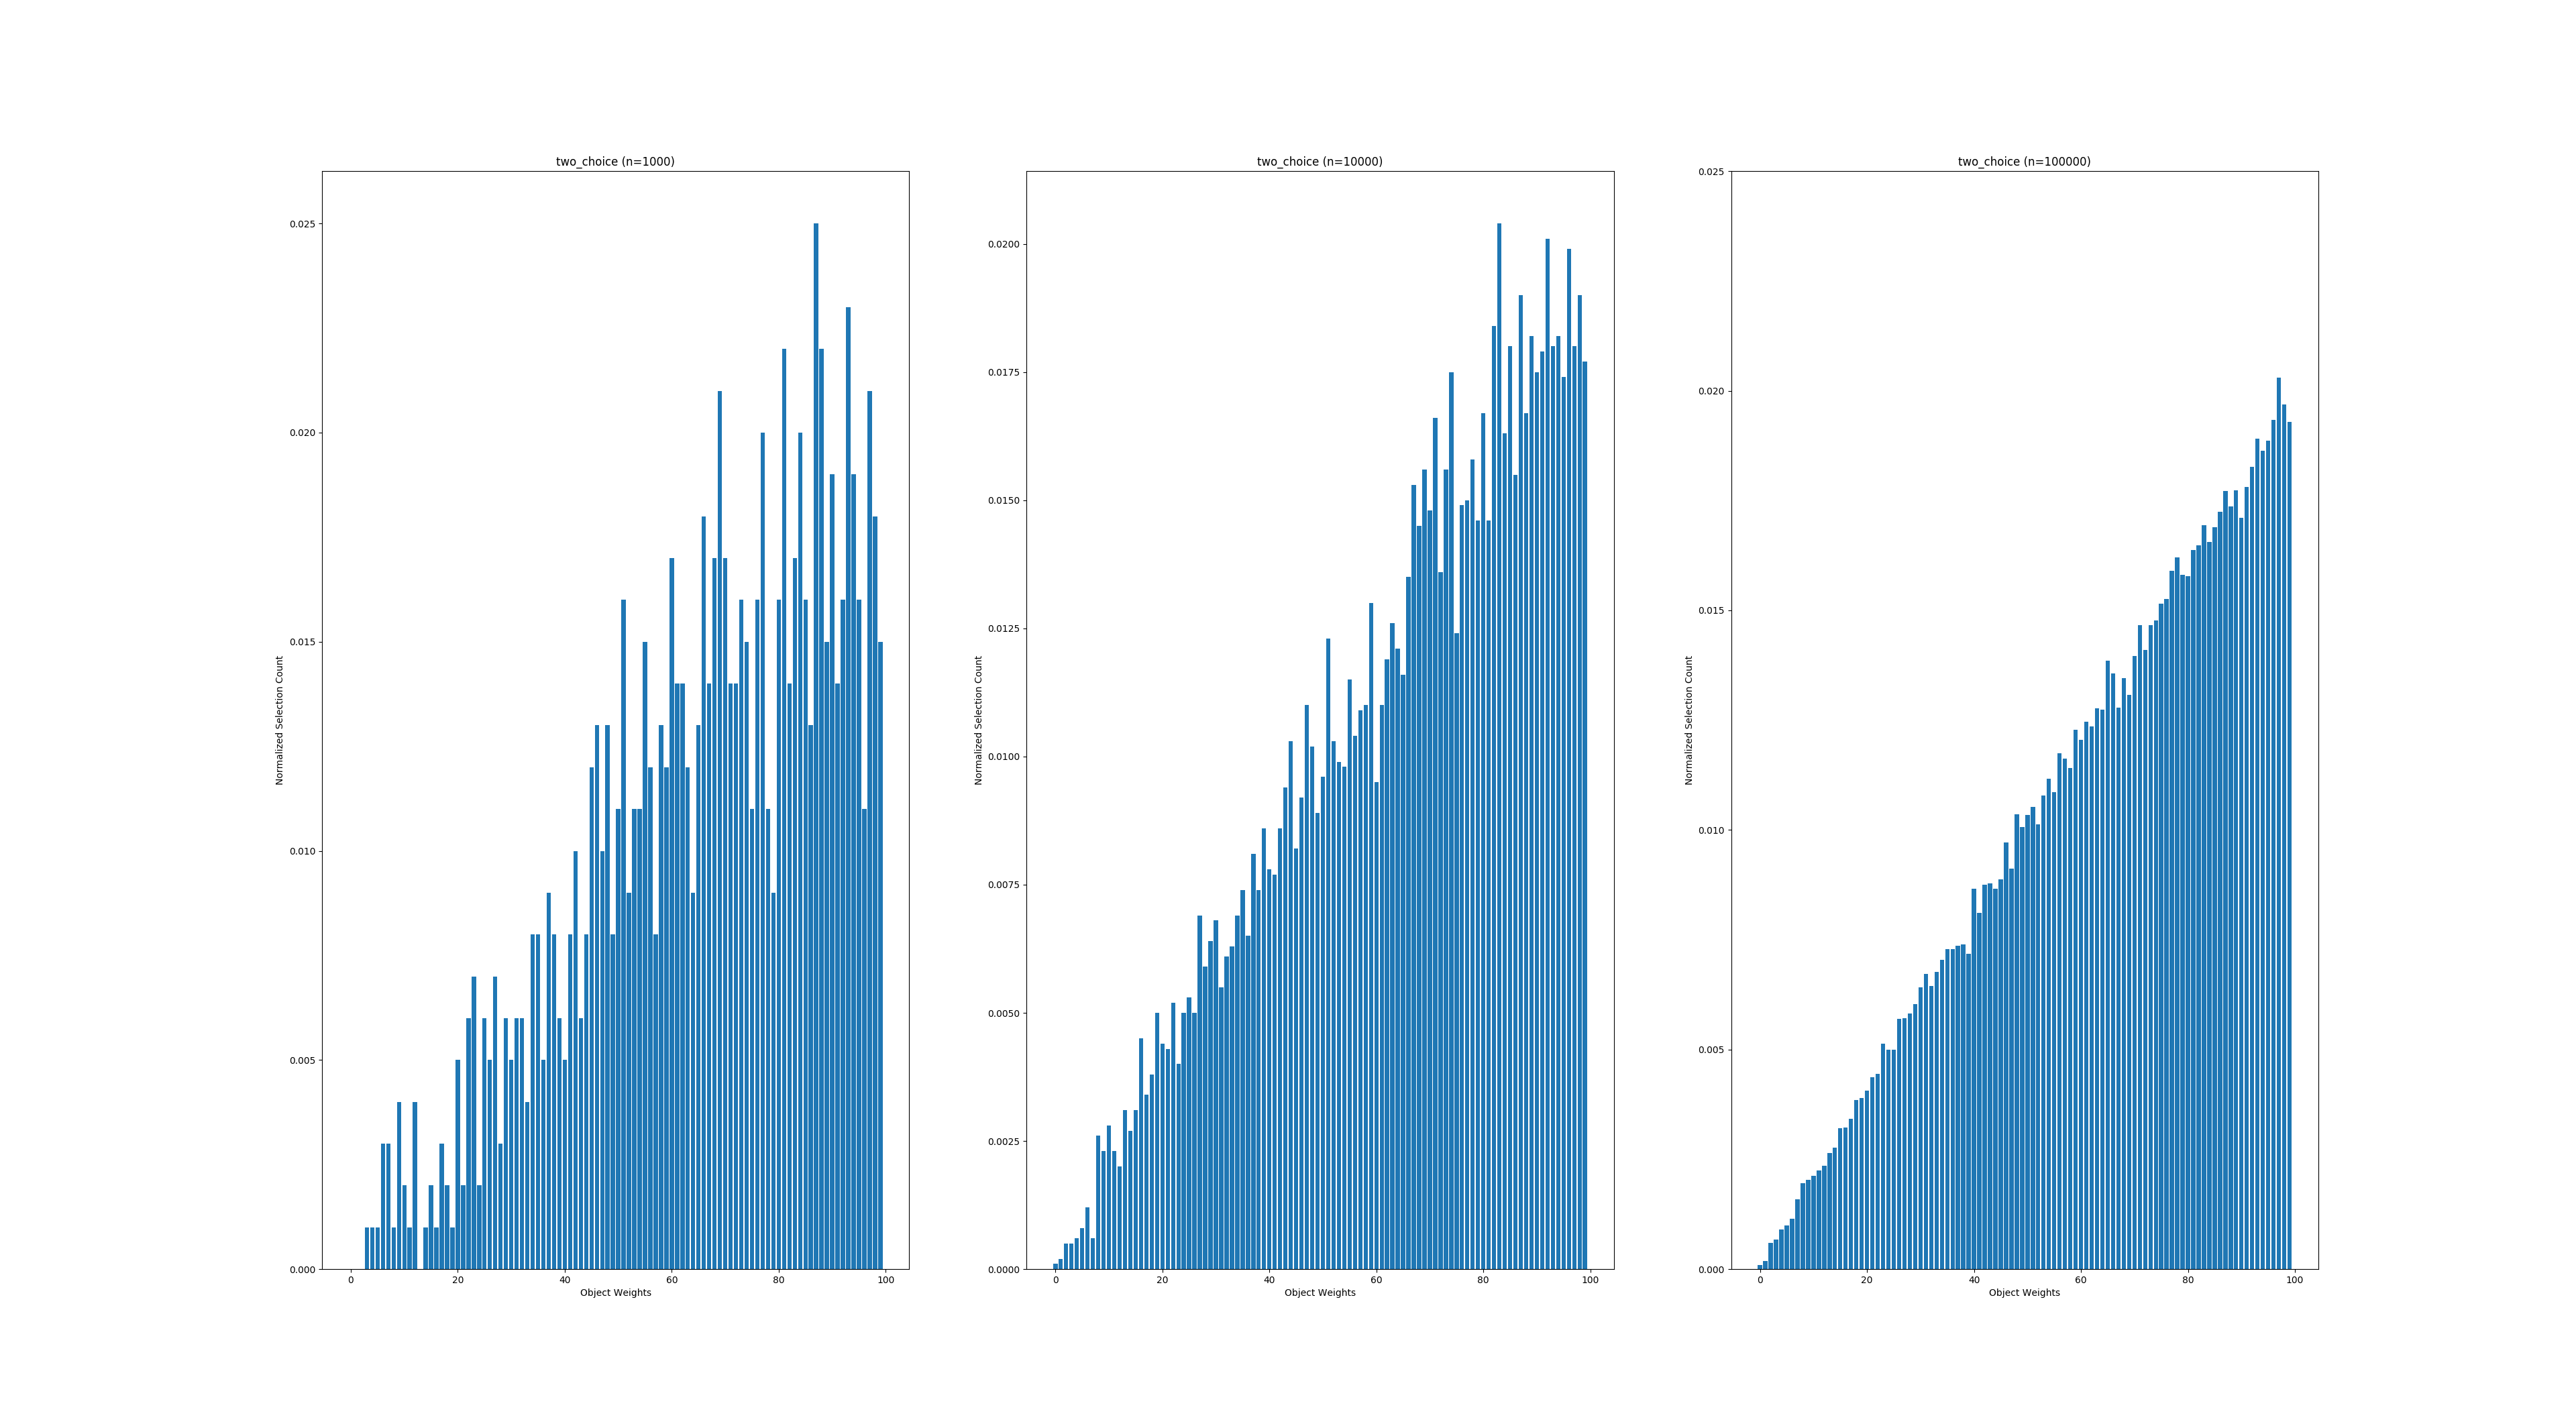
\includegraphics[scale=0.30]{images/herding_two_choice.png} 
      \caption{Histograms generated by simulation of two-choice selection
               using sample sizes of 1e3, 1e4, and 1e5. Object weights
               for the histograms are in the range [1,100].}
      \label{fig:herding_two_choice}
    \end{figure}

    \begin{figure}[h]
      \centering
      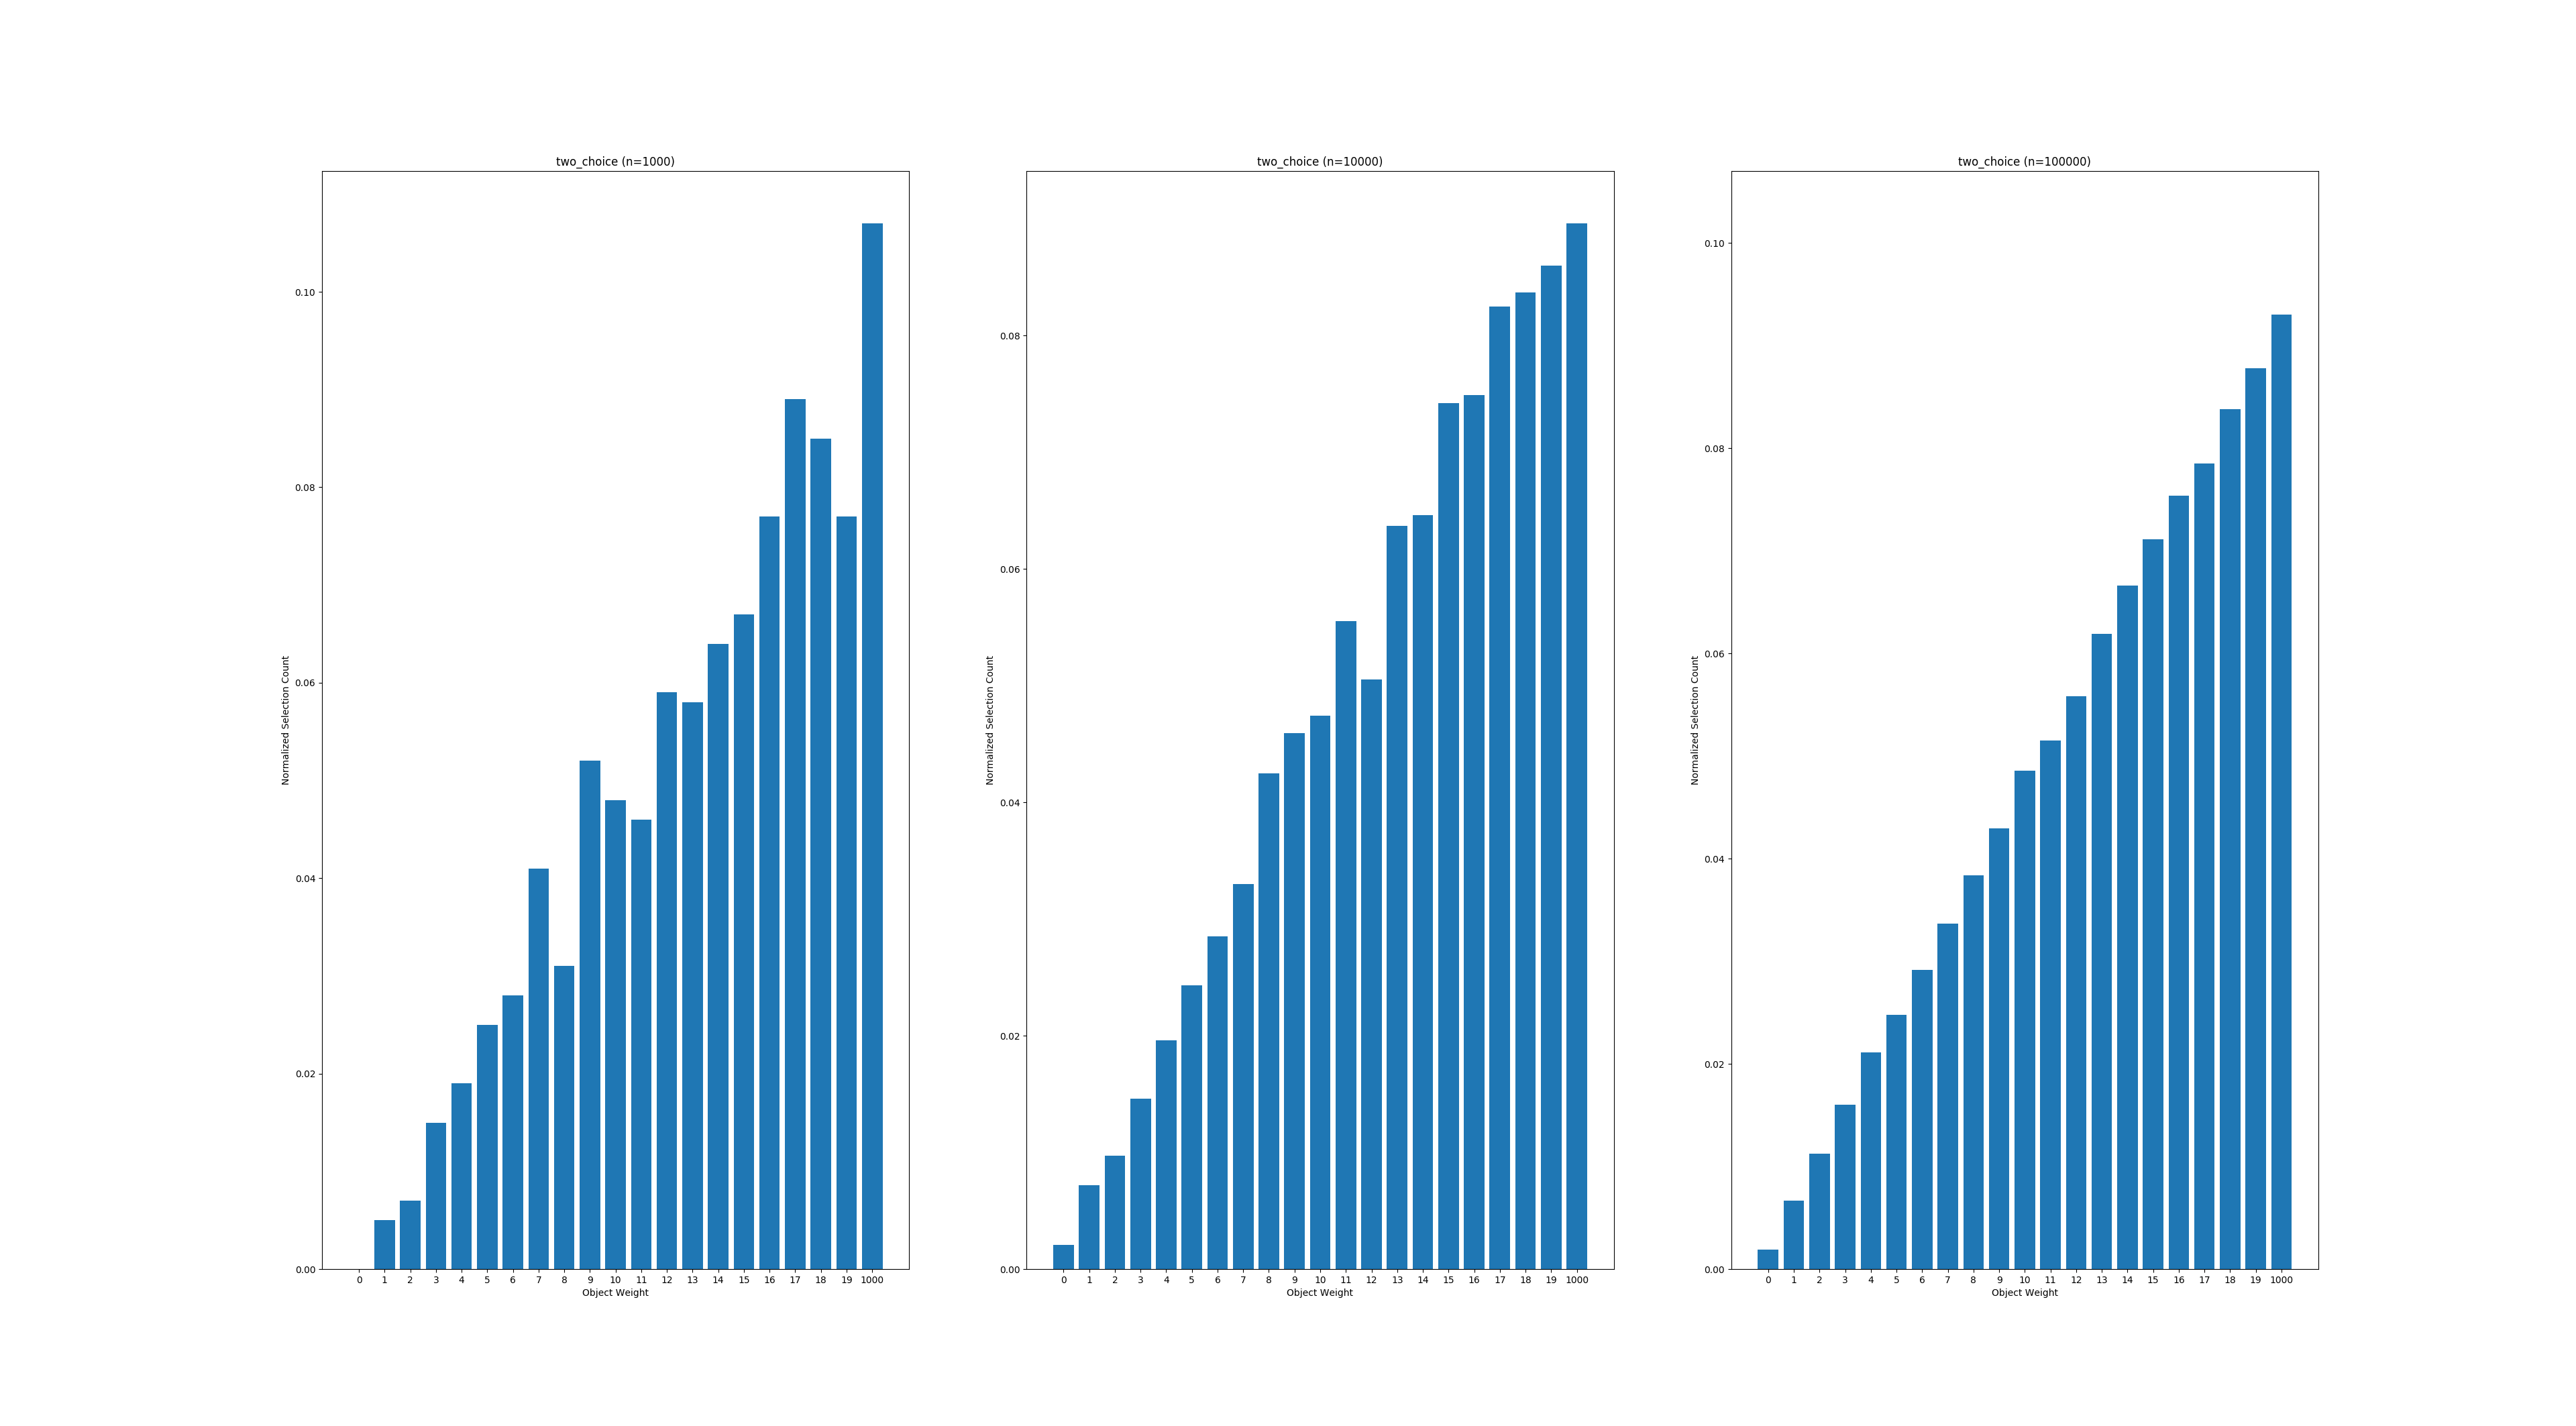
\includegraphics[scale=0.30]{images/pathological_two_choice.png} 
      \caption{Histograms generated by simulation of two-choice selection
               using sample sizes of 1e3, 1e4, and 1e5. Object weights are in
               the range [0,9] with a single outlier of weight 1000 to
               illustrate the effect of herding behavior.}
      \label{fig:pathological_two_choice}
    \end{figure}

    \subsubsection{Uniform Random Selection Simulations}
    Uniform random selection is completely indifferent to object weights.
    Therefore, it exhibits no herding behavior and no usefulness for the
    WeightedVector's sampling, but it is important to include its analysis for
    comparison with other selection algorithms.

    \begin{figure}[h]
      \centering
      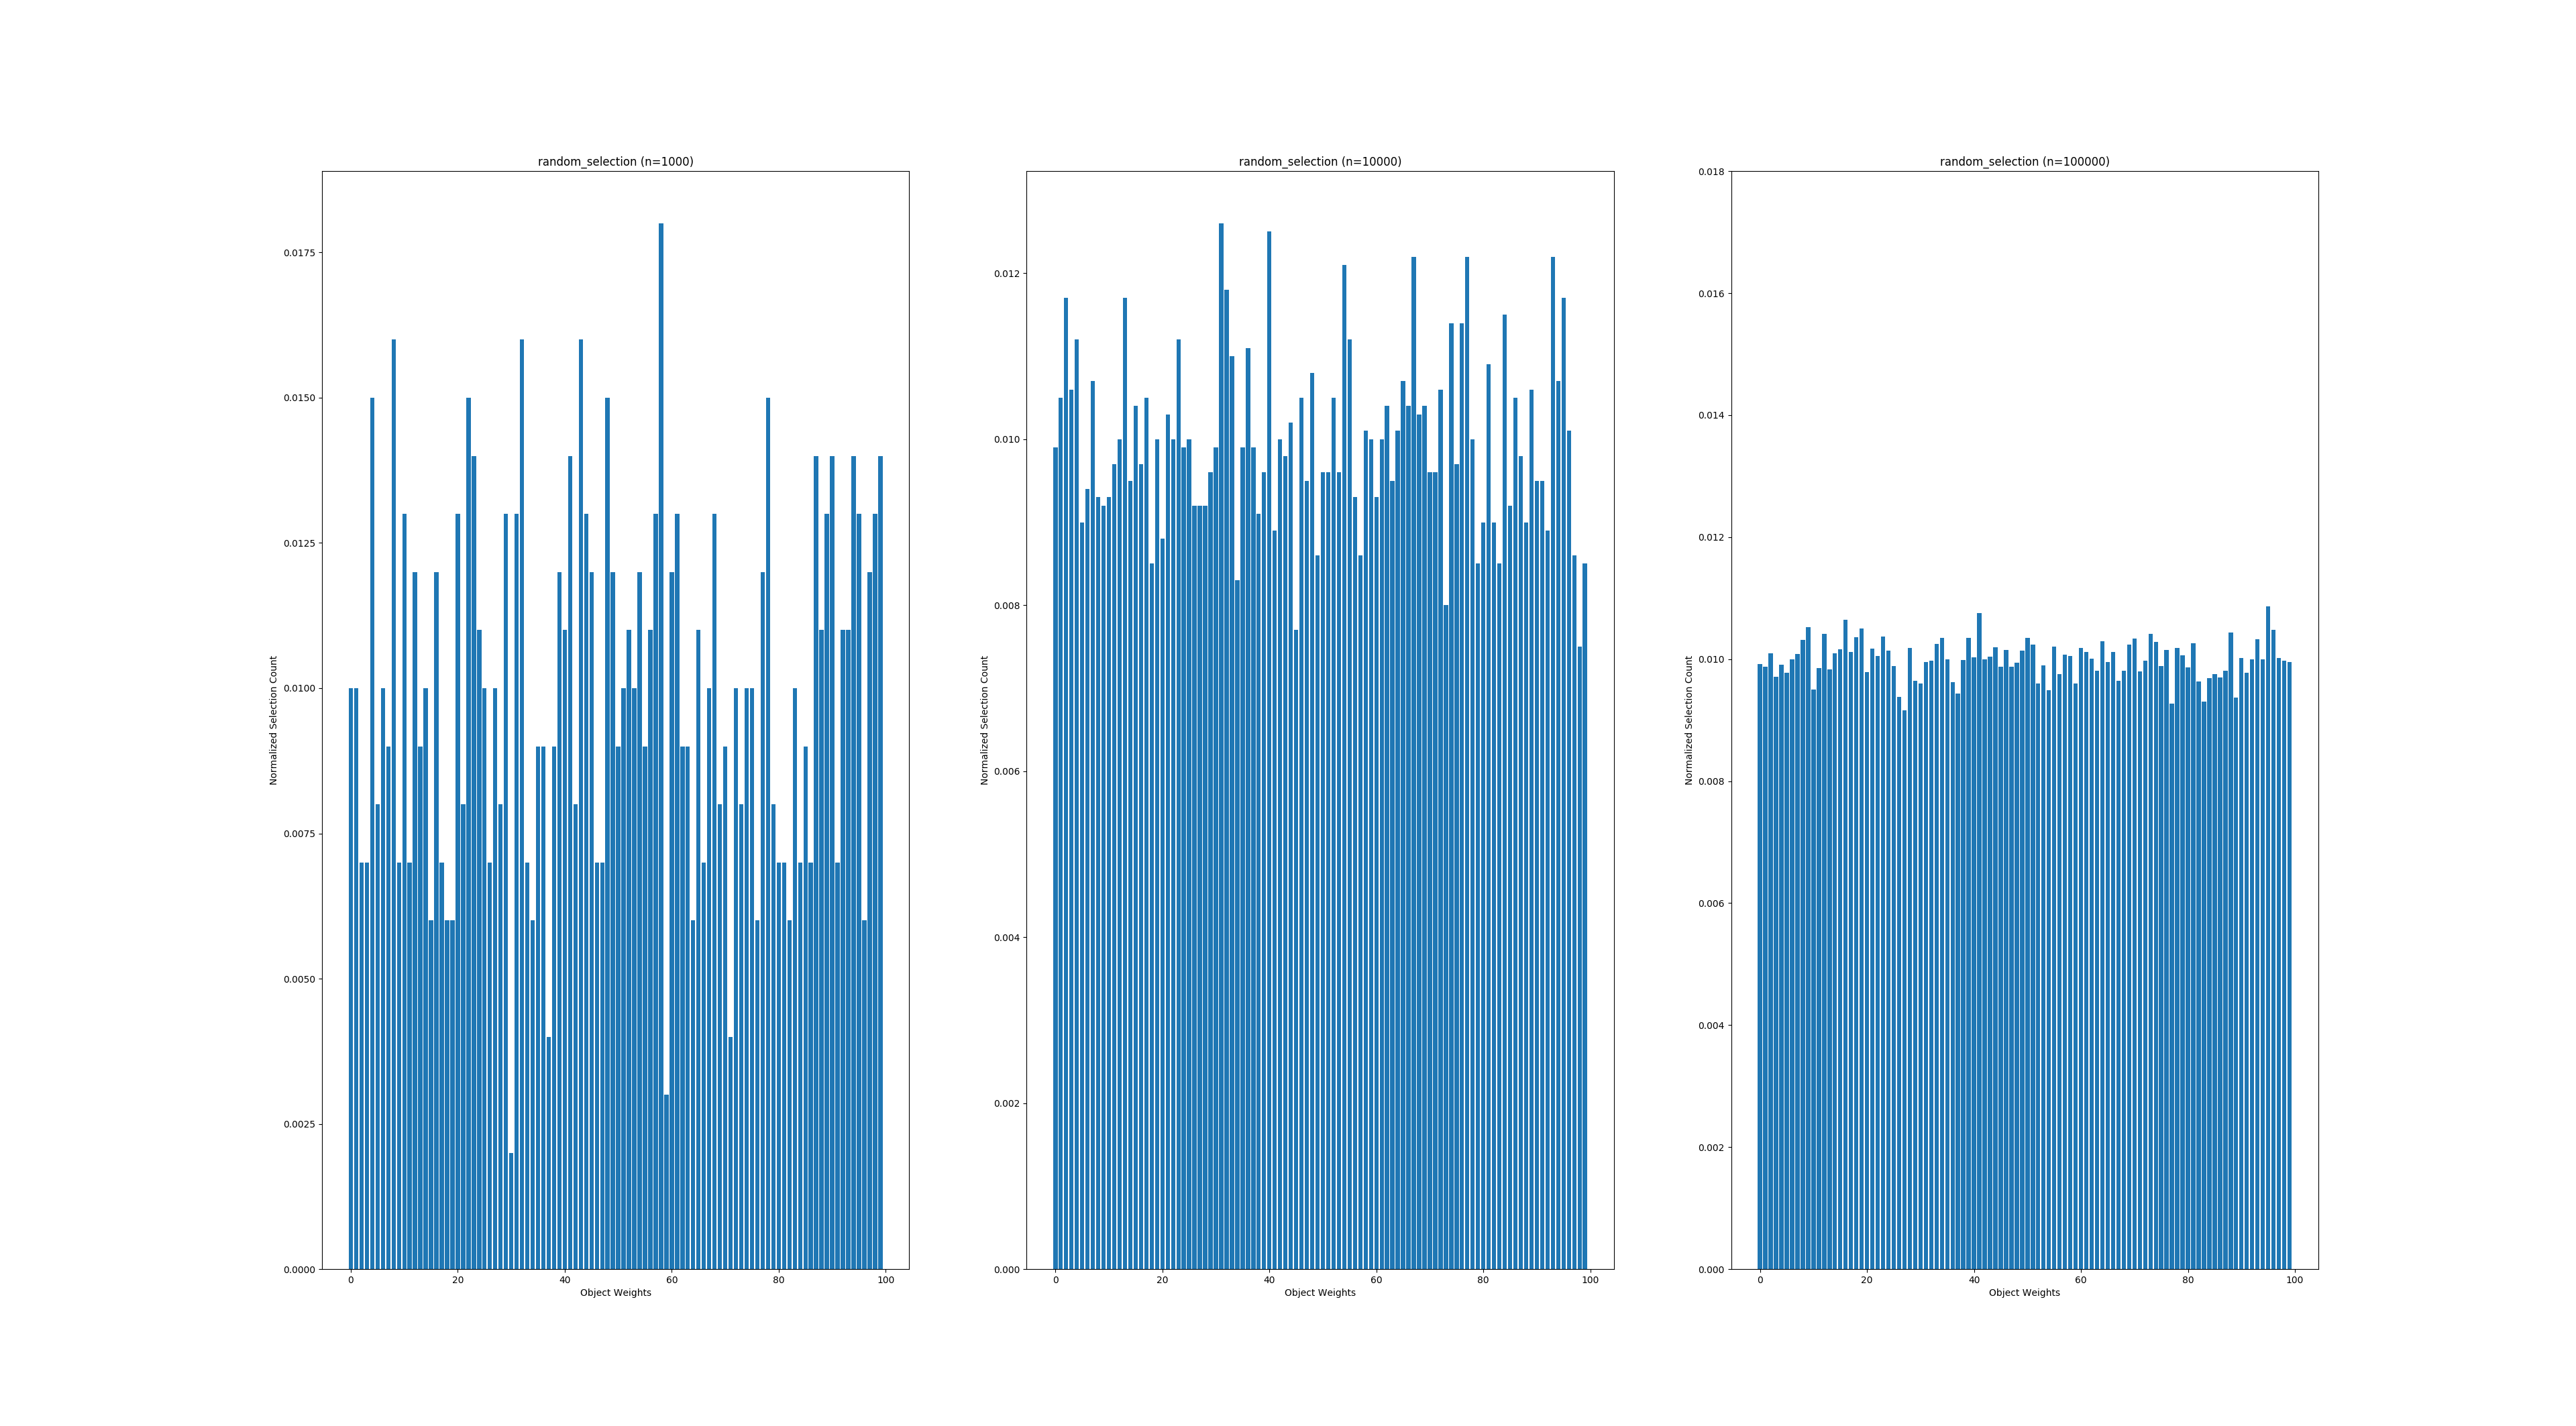
\includegraphics[scale=0.30]{images/herding_random.png} 
      \caption{Histograms generated by simulation of uniform random selection
               using sample sizes of 1e3, 1e4, and 1e5. Object weights
               for the histograms are in the range [1,100].}
      \label{fig:herding_random}
    \end{figure}

    \begin{figure}[h]
      \centering
      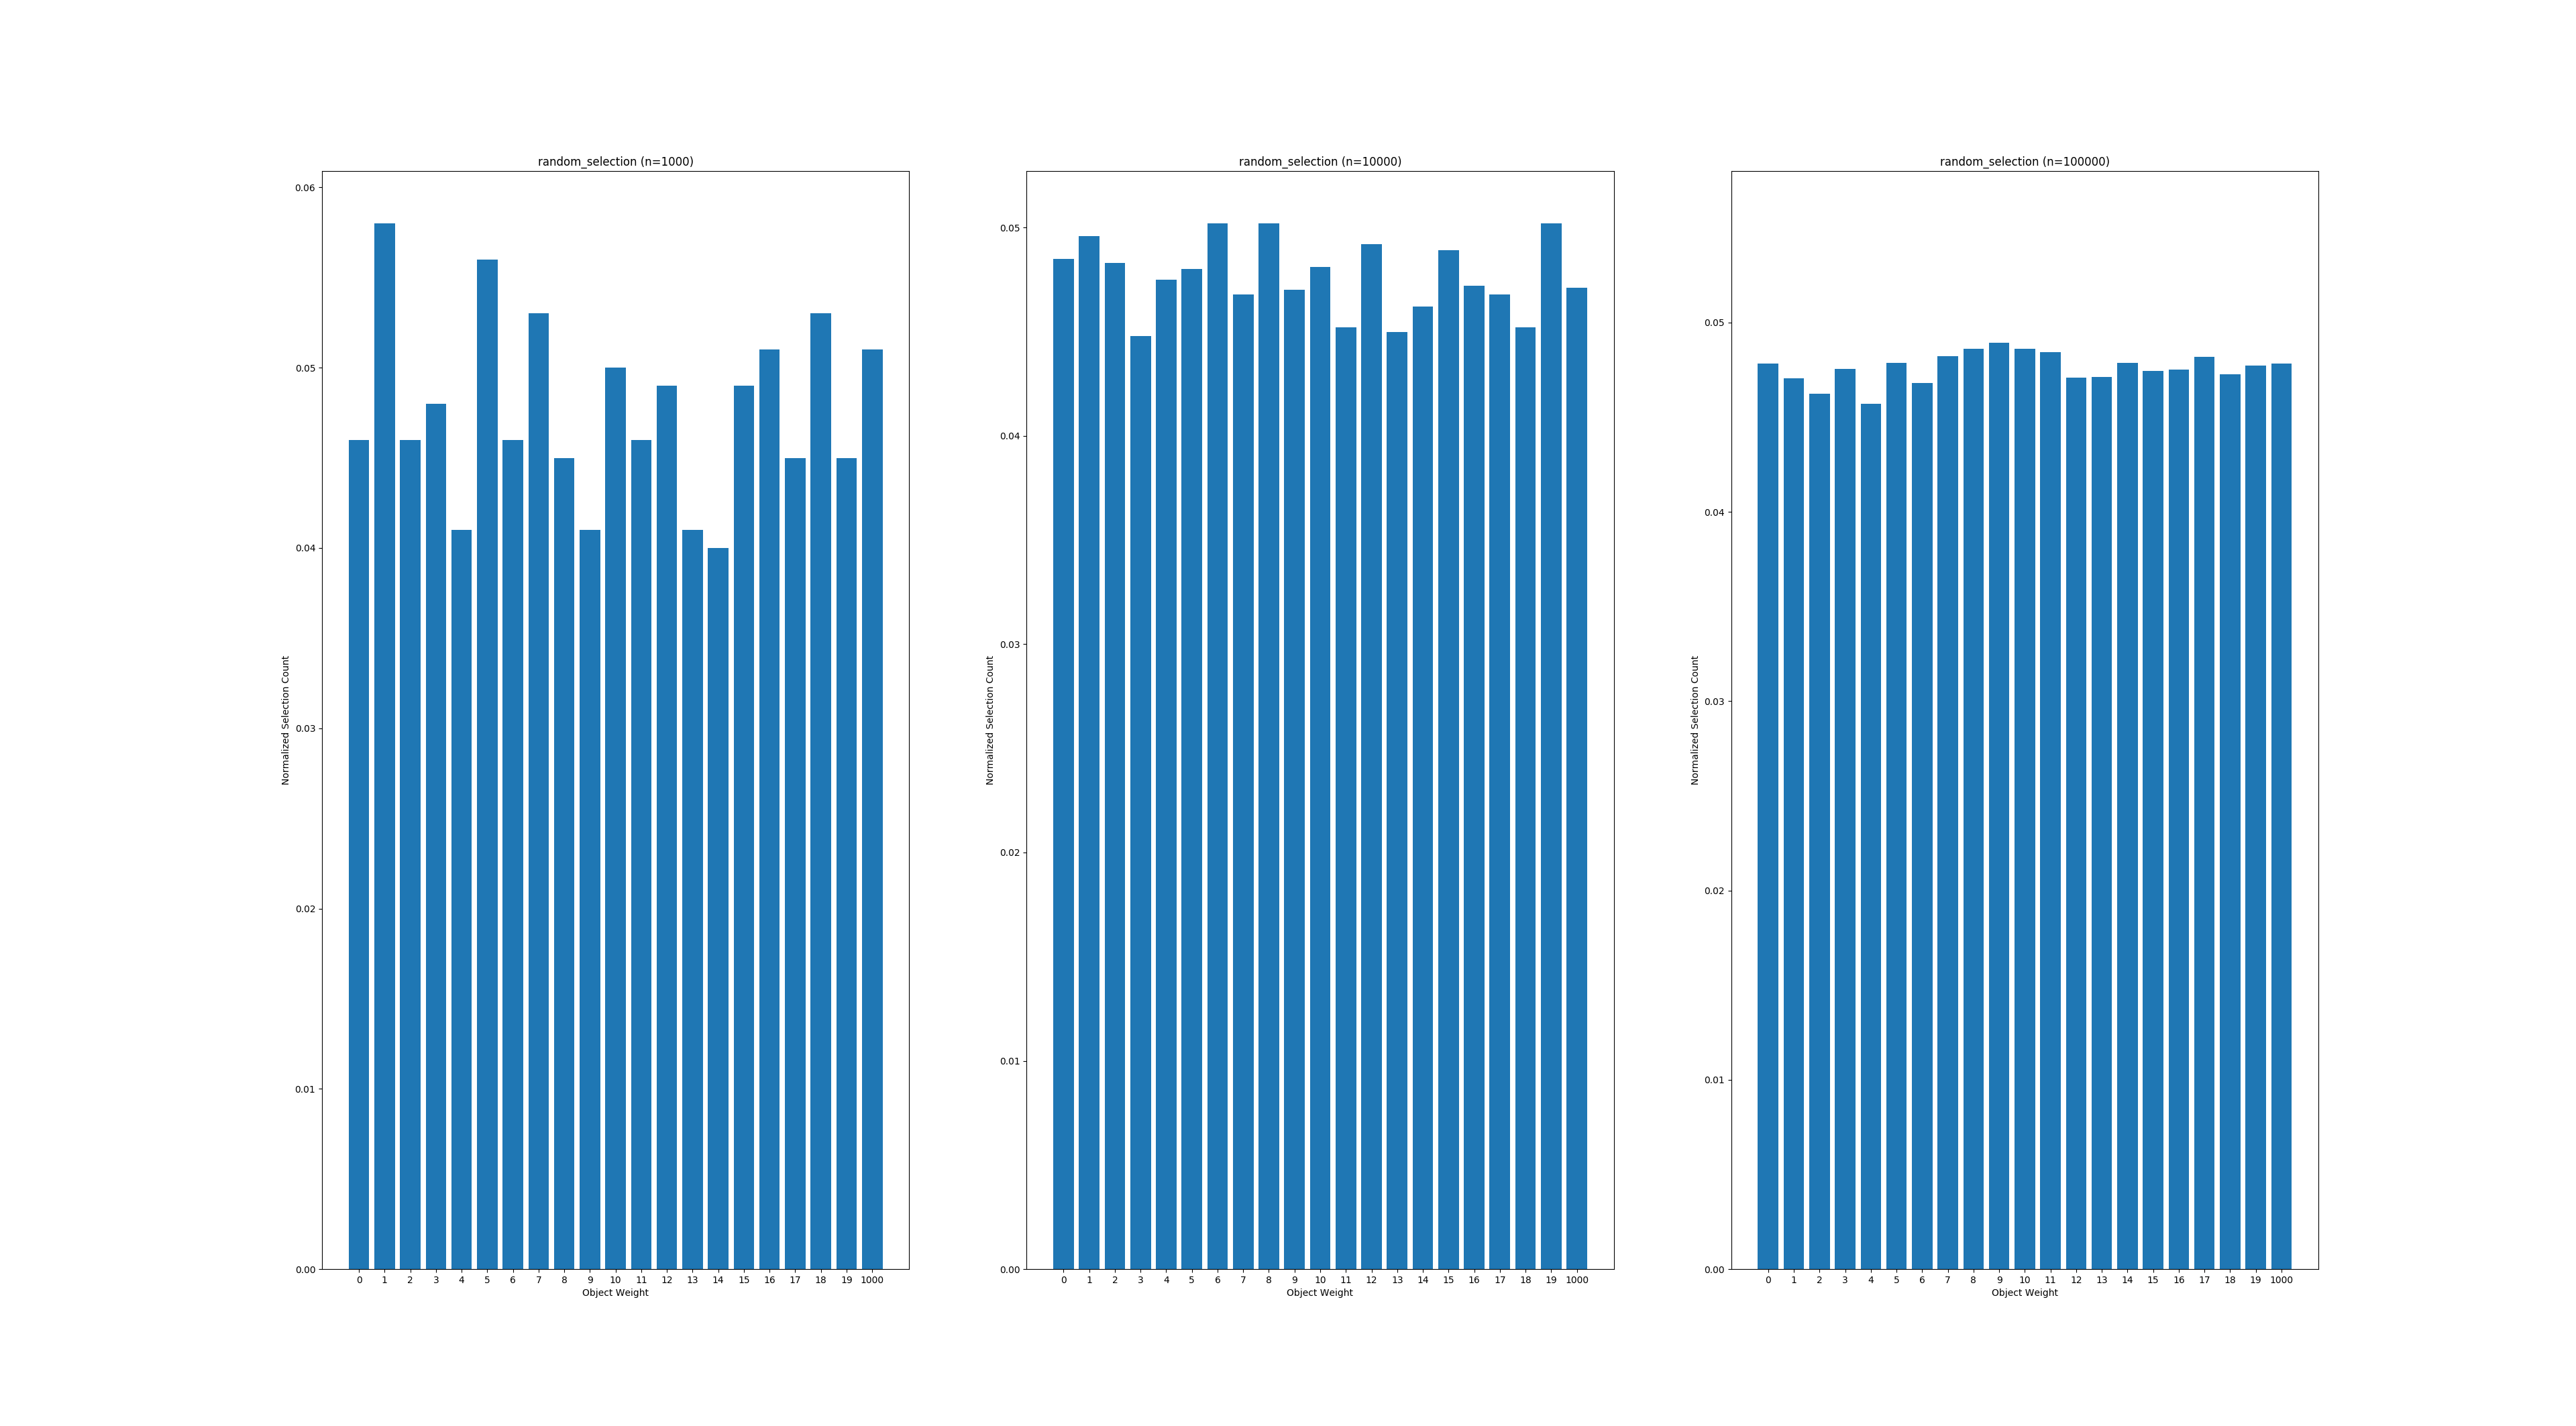
\includegraphics[scale=0.30]{images/pathological_random.png} 
      \caption{Histograms generated by simulation of uniform random selection
               using sample sizes of 1e3, 1e4, and 1e5. Object weights are in
               the range [0,9] with a single outlier of weight 1000 to
               illustrate the effect of herding behavior.}
      \label{fig:pathological_random}
    \end{figure}

    Figure \ref{fig:pathological_truncation} shows that we can expect uniform
    selection probabilities and Figure \ref{fig:pathological_random} confirms
    that we can expect no herding behavior with a uniform random selection
    scheme.

    \subsubsection{Weighted Random Algorithm Scalability Simulations}
    Even though both SUS and truncation selection have $O(N^2)$ time
    complexity, truncation selection is slower than SUS by an order of
    magnitude. This is mainly due to the need for the truncation selection
    algorithm to calculate the top T\% of the set for every selection
    performed. As expected, two-choice and random selections are observed to be
    constant-time algorithms. Two-choice is slightly slower than random
    selection due to the second selection and comparison operation that must
    occur.

    \begin{figure}[h]
      \centering
      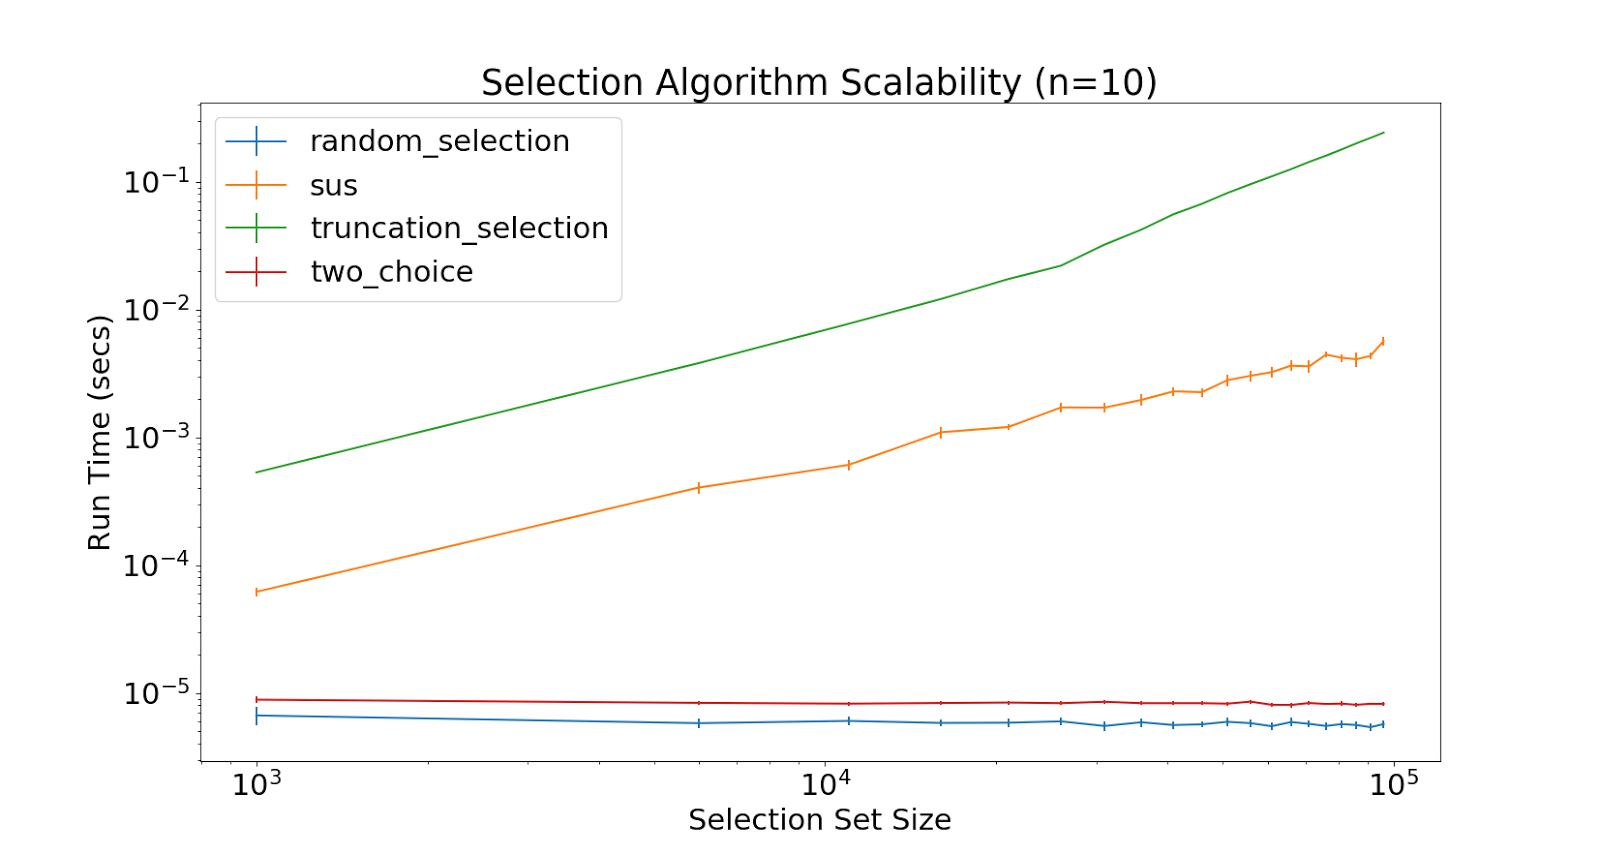
\includegraphics[scale=0.25]{images/random_scalability.png} 
      \caption{Running times of various weight random selection algorithms.
               Each algorithm is run for 10 iterations at each object pool
               size.}
      \label{fig:random_scalability}
    \end{figure}

  \subsection{WeightedVector Class}

  It's necessary to perform repeated weighted sampling of disk IDs, easily, and
  given their fitness values. An object container class is needed similar to a
  C++ STL container \cite{stl} that can also access elements of arbitrary
  types via arbitrary weighted random sampling methods. The WeightedVector
  class was implemented to fulfill this requirement. 

  Upon instantiation of the WeightedVector class, a fitness function is
  provided to store the fitness values of all objects internally. The
  WeightedVector class has implemented insertion, removal, and weighted random
  sampling of objects of some arbitrary type, $T$, based on the object's
  fitness value as a weight.

  The set of objects and their fitness values are stored in $std::vector$
  objects , one for the object references stored in the WeightedVector and one
  for their corresponding fitness values. The objects and their corresponding
  fitness values share an index into their respective internal vectors.

    \subsubsection{Public Interface}

     \begin{verbatim}
       WeightedVector(const std::function<double(const T)>)
     \end{verbatim}

     The WeightedVector class is instantiated by providing a fitness function
     that accepts a reference to an object of type \emph{T} and returns a
     fitness value that is of type \emph{double}. The provided fitness function
     is used to create a mapping between inserted objects and their
     corresponding fitness values for sampling.

     The WeightedVector class asserts that the fitness function returns positive
     values.

     \begin{verbatim}
       void EmplaceBack(const T& element)
     \end{verbatim}

     The EmplaceBack function constructs and inserts an object of type
     \emph{T} at the end of the vector. This increases the WeightedVector's
     size by 1.

     \begin{verbatim}
       bool Empty()
     \end{verbatim}

     Returns true if the WeightedVector is of size 0.

     \begin{verbatim}
       void Clear()
     \end{verbatim}

     Resets all state in the WeightedVector object, sets the size to 0, and
     clears all internal vectors.

     \begin{verbatim}
       T& Sample()
     \end{verbatim}

     Returns a reference to an object stored inside of the WeightedVector.
     Objects are sampled via weighted random selection and subsequent calls to
     Sample are guaranteed not to return the same object unless Reset is called
     before sampling again. The WeightedVector class asserts that Sample is not
     called more times than the size of the WeightedVector.

     \begin{verbatim}
       void Reset()
     \end{verbatim}

     Resets the sampling state of the WeightedVector, allowing sampled objects
     to be eligible for selection in subsequent Sample calls.

     \begin{verbatim}
       size_t size()
     \end{verbatim}

     Returns the size of the WeightedVector.

    \subsubsection{Weighted Vector Internals}

    Internally, the WeightedVector class keeps 3 different std:vector objects
    to keep track of sampling state and the object-to-fitness value mapping.
    There is the inner\_vector\_ variable which stores the objects
    inserted via EmplaceBack(), the weights\_ variable which stores the
    fitness values of all objects in the inner\_vector\_, and the
    sampling\_weights\_ variable which is identical to weights\_
    except that objects weights are set to 0 when sampled. This allows us to
    exclude objects from being sampled multiple times with time complexity
    $O(1)$, since a weight of 0 gives a probability of 0 for sampling using
    Stochastic Universal Sampling as shown in the example below.

    Before sampling, we have identical weights\_ and sampling\_weights\_
    accompanying an inner\_vector\_ of objects:

    \begin{center}
      \begin{tabular}{ | l | c | c | c | r | }
        \hline
        \verb|inner_vector_| & $A$ & $B$ & $C$ & $D$ \\ \hline
        \verb|weights_| & 1 & 3 & 3 & 7 \\ \hline
        \verb|sampling_weights_| & 1 & 3 & 3 & 7 \\ \hline
        \hline
      \end{tabular}
    \end{center}

    Suppose we then call Sample() on the WeightedVector and it returns $D$. The
    probability of this event is 0.5, so to maintain sampling state within the
    WeightedVector, the weight associated with object $D$ is set to zero:

    \begin{center}
      \begin{tabular}{ | l | c | c | c | r | }
        \hline
        \verb|inner_vector_| & $A$ & $B$ & $C$ & $D$ \\ \hline
        \verb|weights_| & 1 & 3 & 3 & 7 \\ \hline
        \verb|sampling_weights_| & 1 & 3 & 3 & 0 \\ \hline
        \hline
      \end{tabular}
    \end{center}

    If we call Sample() again, it is not possible to return $D$ since its
    sampling weight is now zero. The probabilities of returning $A$, $B$, or
    $C$ in subsequent calls to Sample() are $\frac{1}{7}$, $\frac{3}{7}$, and
    $\frac{3}{7}$ respectively. Suppose two more calls to Sample() lead to the
    following state:

    \begin{center}
      \begin{tabular}{ | l | c | c | c | r | }
        \hline
        \verb|inner_vector_| & $A$ & $B$ & $C$ & $D$ \\ \hline
        \verb|weights_| & 1 & 3 & 3 & 7 \\ \hline
        \verb|sampling_weights_| & 0 & 3 & 0 & 0 \\ \hline
        \hline
      \end{tabular}
    \end{center}

    We may only call Sample() one more time without triggering an assertion
    failure and the WeightedVector is obligated to return $D$. The only way to
    restore sampling state is to call Reset(). A Reset call simply copies
    weights\_ into sampling\_weights\_ and all objects are eligible for
    sampling again:

    \begin{center}
      \begin{tabular}{ | l | c | c | c | r | }
        \hline
        \verb|inner_vector_| & $A$ & $B$ & $C$ & $D$ \\ \hline
        \verb|weights_| & 1 & 3 & 3 & 7 \\ \hline
        \verb|sampling_weights_| & 1 & 3 & 3 & 7 \\ \hline
        \hline
      \end{tabular}
    \end{center}


    \subsubsection{Weighted Vector Unit Testing}

    The WeightedVector class' unit test has four phases:

    \begin{enumerate}
      \item Test Average() functionality
      \item Test there are no duplicate samples
      \item Test sampling with uniform probabilities
      \item Test sampling with non-uniform probabilities
    \end{enumerate}

    The testing of the Average() function's behavior includes simply adding all
    zeros, all ones, and monotonically increasing integers in the range
    $[0,N]$. For each phase, we verify that the reported average is 0, 1, and
    $\frac{N(N-1)}{2N}$ respectively.  

    Verification that there are no duplicate samples involves adding
    monotonically increasing integers in the range $[0,N]$, inserting all
    sampled elements into a hash set, and verifying that the size of the hash
    set is equal to the size of the WeightedVector.

    To test sampling of objects with uniform and non-uniform weights, I add
    monotonically increasing integers in the range $[0,N]$ to the
    WeightedVector. The fitness function provided for the uniform test simply
    returns a weight of 1 for all objects inserted into the WeightedVector.
    Elements are then sampled and Reset() is called for a number of times
    several orders of magnitude larger than the number of elements. Each
    sampled element's number of times being selected is tracked in a test-local
    hash map. We then calculate the actual selection probability of each
    element in the WeightedVector with the expected value and verify the
    difference is within an acceptable tolerance. For the uniform test, we
    expect all integers to be sampled roughly the same amount and for the
    non-uniform test, we expect larger integers to be sampled an amount of
    times proportional to their value.

  \subsection{Replica Selection Changes}
    
  Stargate was modified to store disk IDs in a WeightedVector rather than a
  \verb|std::vector|. When considering a disk for candidacy, rather than
  shuffling the \verb|std::vector| and iterating through each disk until enough
  replica targets are found, we call \verb|WeightedVector::Sample()| until
  enough replica targets are found. All of Stargate's replica placement logic
  is untouched and I've simply modified the order in which candidate disks are
  considered.
      
%%%%%%%%%%%%%%%%%%%%%%%%%%%%%%%%%%%%%%%%%%%%%%%%%%%%%%%%%%%%%%%%%%%%%%%%%%%%%%%

\section{Evaluation and Results}

The experiments below seek to measure the effect of the additive and
multiplicative term fitness functions on both the tier utilization of each node
and the queue lengths of disks residing on those nodes compared with uniform
random selection.

  \subsection{Experimental Setup}

  The replica selection schemes were evaluated using a NX-1350 for evaluating
  the disk fullness and a NX-3-node cluster). Each node contains a single 300GB
  SSD and 4 HDDs 1TB in size. When evaluating the new replica disk selection
  framework, two heterogeneous workload scenarios are tested:
 
  \begin{enumerate}
    \item Two worker VMs on separate nodes running a workload with low
          outstanding ops.
    \item Two worker VMs on separate nodes with running a
          workload with high outstanding ops.
  \end{enumerate}
 
  \subsection{Fio and Write Patterns}

  When generating I/O in these experiments, Fio is used on the worker VMs. Fio,
  short for Flexible IO, is an I/O workload generator that can take
  configuration files to specify the parameters of a test. On each worker VM,
  fio is used to generate a sequential write workload that completely fills the
  cluster's hot-tier. I choose to use exclusively sequential writes for all
  tests because they are the default for fio tests and the purpose of these
  experiments is to generate new replicas in a consistent manner. For the
  purposes of replica placement, the Nutanix file system does not distinguish
  targets based on the write pattern that generatred an extent group.

  \subsection{Tier Utilization Experiments}

  The tier utilization experiments define the hot-tier deviation,
  $d_{hot tier}$, as the average SSD utilization percentage of the nodes
  running a workload, $u_{w}$, subtracted by the SSD utilization percentage of
  the node without a workload, $u_{o}$:
  
  \begin{equation}
    d_{hot\ tier} = \frac{u_{w1} + u_{w2}}{u_{o}}
  \end{equation}
  
  Ideally, the idle node would absorb the majority of secondary replicas from
  the running workloads. However, uniform random selection causes only 50\% of
  secondary replicas to go to the idle node even though it can potentially
  handle more work due to the fact that it does not have to service a local
  workload. In a uniform random replica selection scheme, we expect the
  nodes running a workload have to bear 100\% of their own primary replicas and
  50\% of secondary replicas from the other worker node. This causes total SSD
  utilization to be skewed towards the worker nodes and for this skew to grow
  as the tests run. This is indicated by higher $d_{hot\ tier}$ values. We
  expect a more sophisticated replica selection scheme to minimize
  $d_{hot\ tier}$ by biasing secondary replicas towards the idle node and
  limiting the skew.

  % TODO: should I include fio scripts here, in some appendix, or in the user
  % guide?

    \subsubsection{Low Outstanding Operation Results}

    \begin{figure}[h]
      \centering
      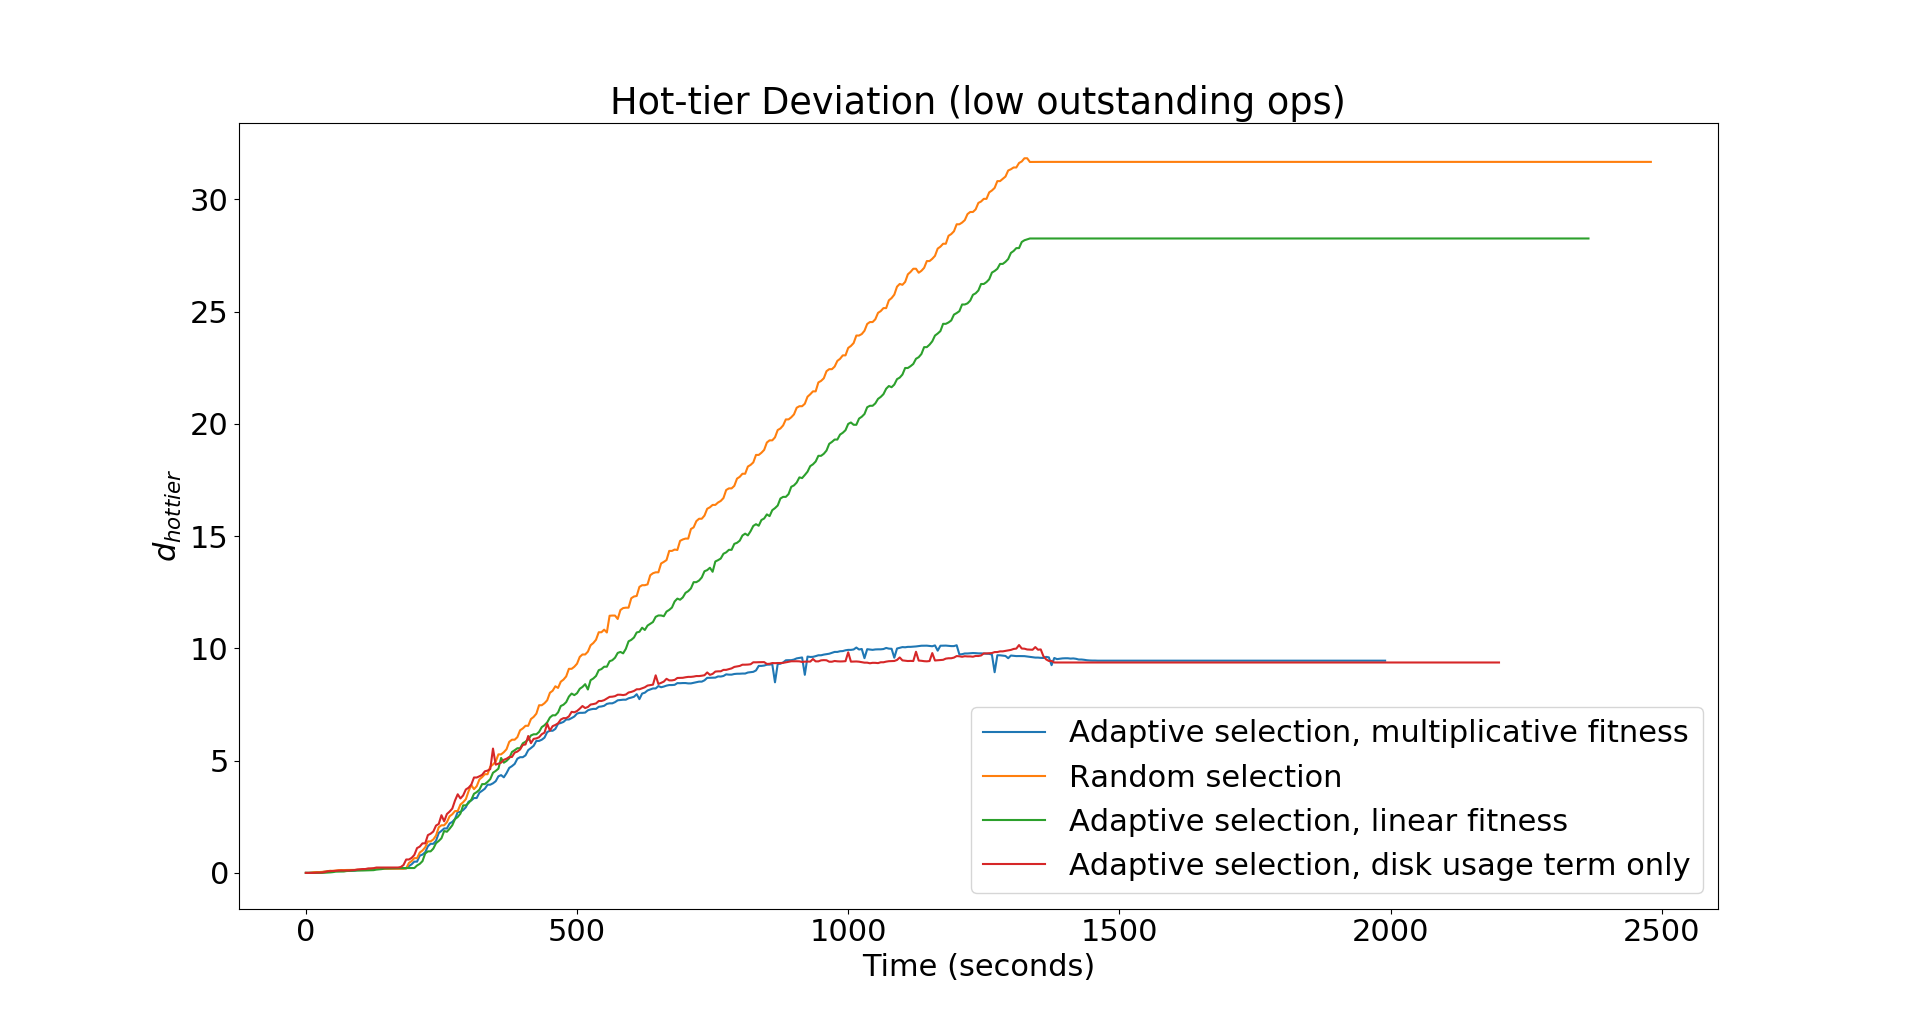
\includegraphics[scale=0.30]{images/low_outstanding_exp.png} 
      \caption{$d_{hot\ tier}$ values over time for low outstanding I/O
               operations.}
      \label{fig:low_outstanding_tier_disparity}
    \end{figure}

    Figure \ref{fig:low_outstanding_tier_disparity} shows the results of a
    workload with only a single outstanding operation. This causes the queue
    length reported by Stargate to be at most 1, resulting in the fitness
    function's queue length term to be roughly constant and approximately 1.
    
    We can see that the additive fitness function does not minimize the
    hot-tier deviation as well as the multiplicative. This is because an
    additive fitness function's behavior varies depending on the weight chosen
    for the queue length term. By default, the linear fitness function
    gives equal weight to both the disk fullness and queue length terms;
    however, for one run of this experiment the queue length term was given no
    weight. Linear fitness that gives equal weight to both terms does not
    reduce skew by very much while giving no weight to the queue length term
    keeps all nodes' usages within 10\% of each other. This is because the
    queue length term is contributing the maximum amount possible to the
    fitness value due to the consistently low queue length values. We can
    illustrate this by defining a disk selection bias, $b_r$, as the
    probability some disk, $d$, will be selected when compared with another
    disk, $d'$ whose utilization is 10\% higher and queue length value is
    identical. Given a fitness function, $f$, we can calculate $b_r$ as
    follows:

    \begin{equation}
      b_r = \frac{f(d)}{f(d) + f(d')}
    \end{equation}

    Figures \ref{fig:bias_max_qlen} and \ref{fig:bias_min_qlen} show the disk
    selection biases for very large and very small queue lengths respectively.

    \begin{figure}[h]
      \centering
      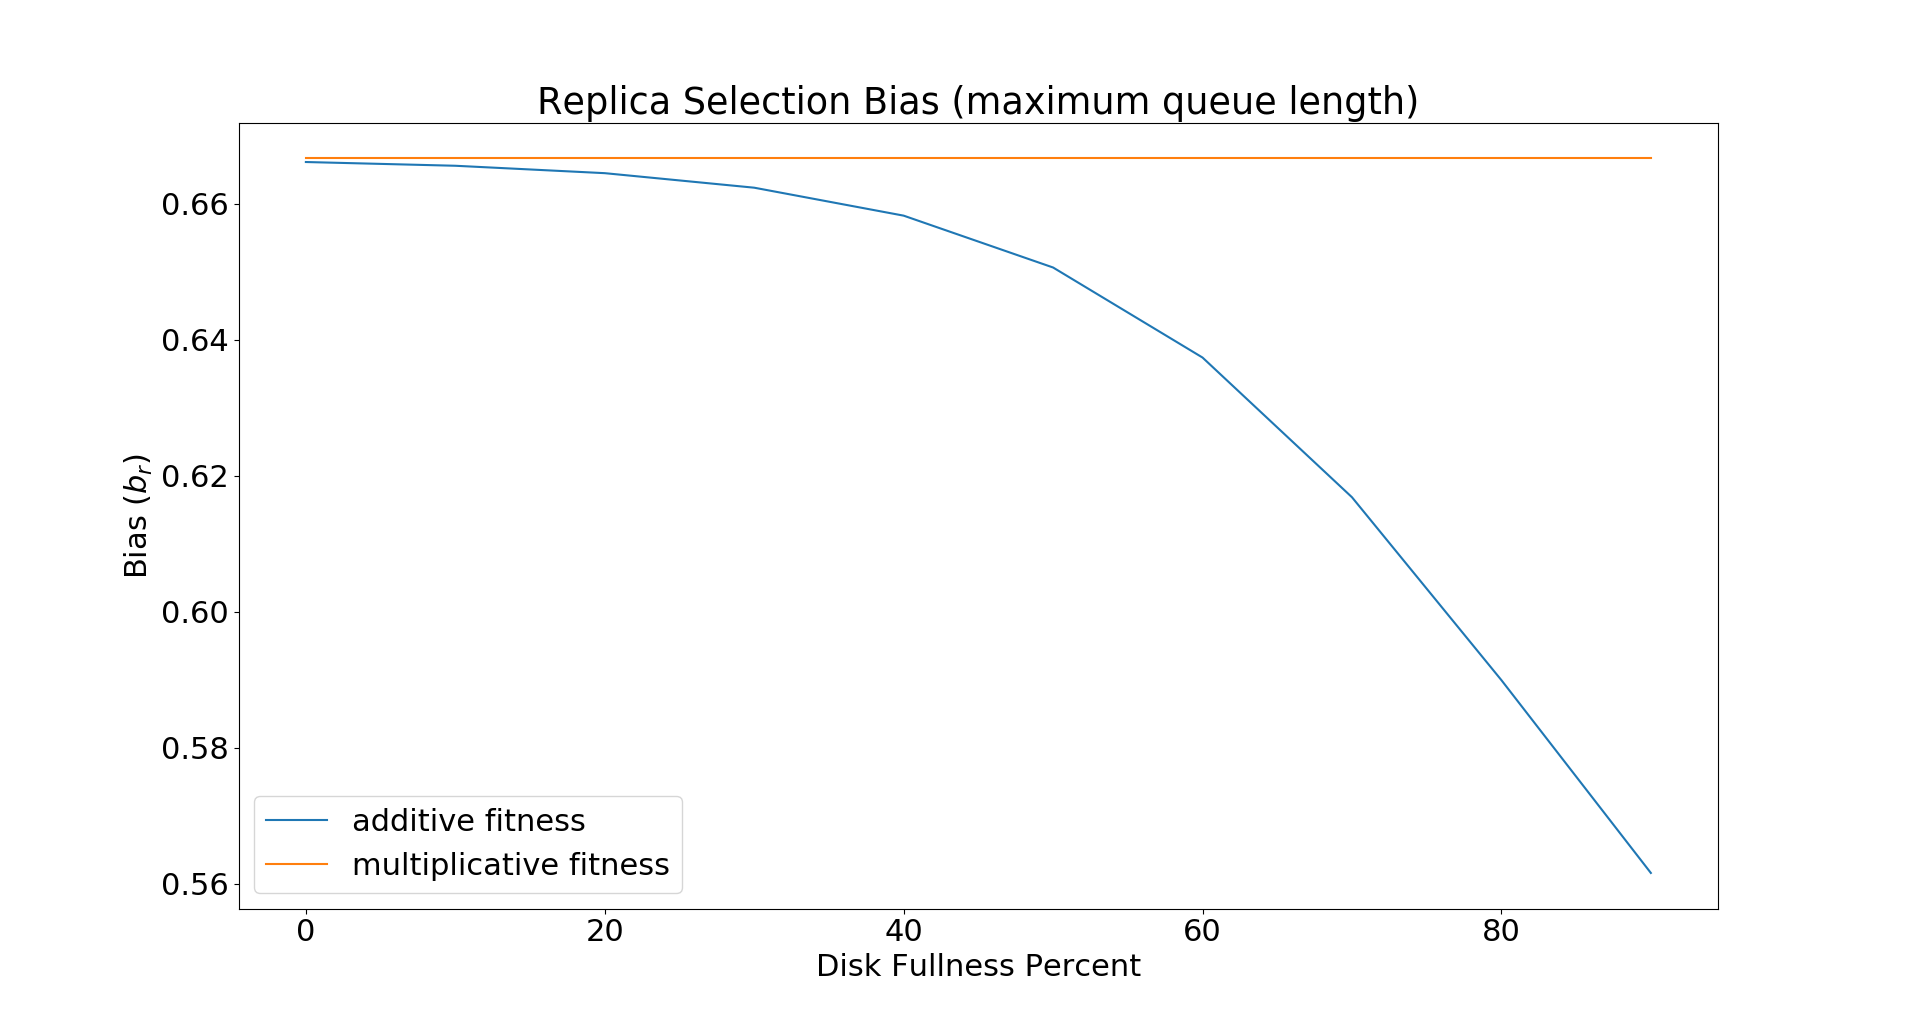
\includegraphics[scale=0.30]{images/replica_selection_bias_max_qlen.png} 
      \caption{$b_r$ values with static queue lengths at the fitness
               function ceiling values.}
      \label{fig:bias_max_qlen}
    \end{figure}

    \begin{figure}[h]
      \centering
      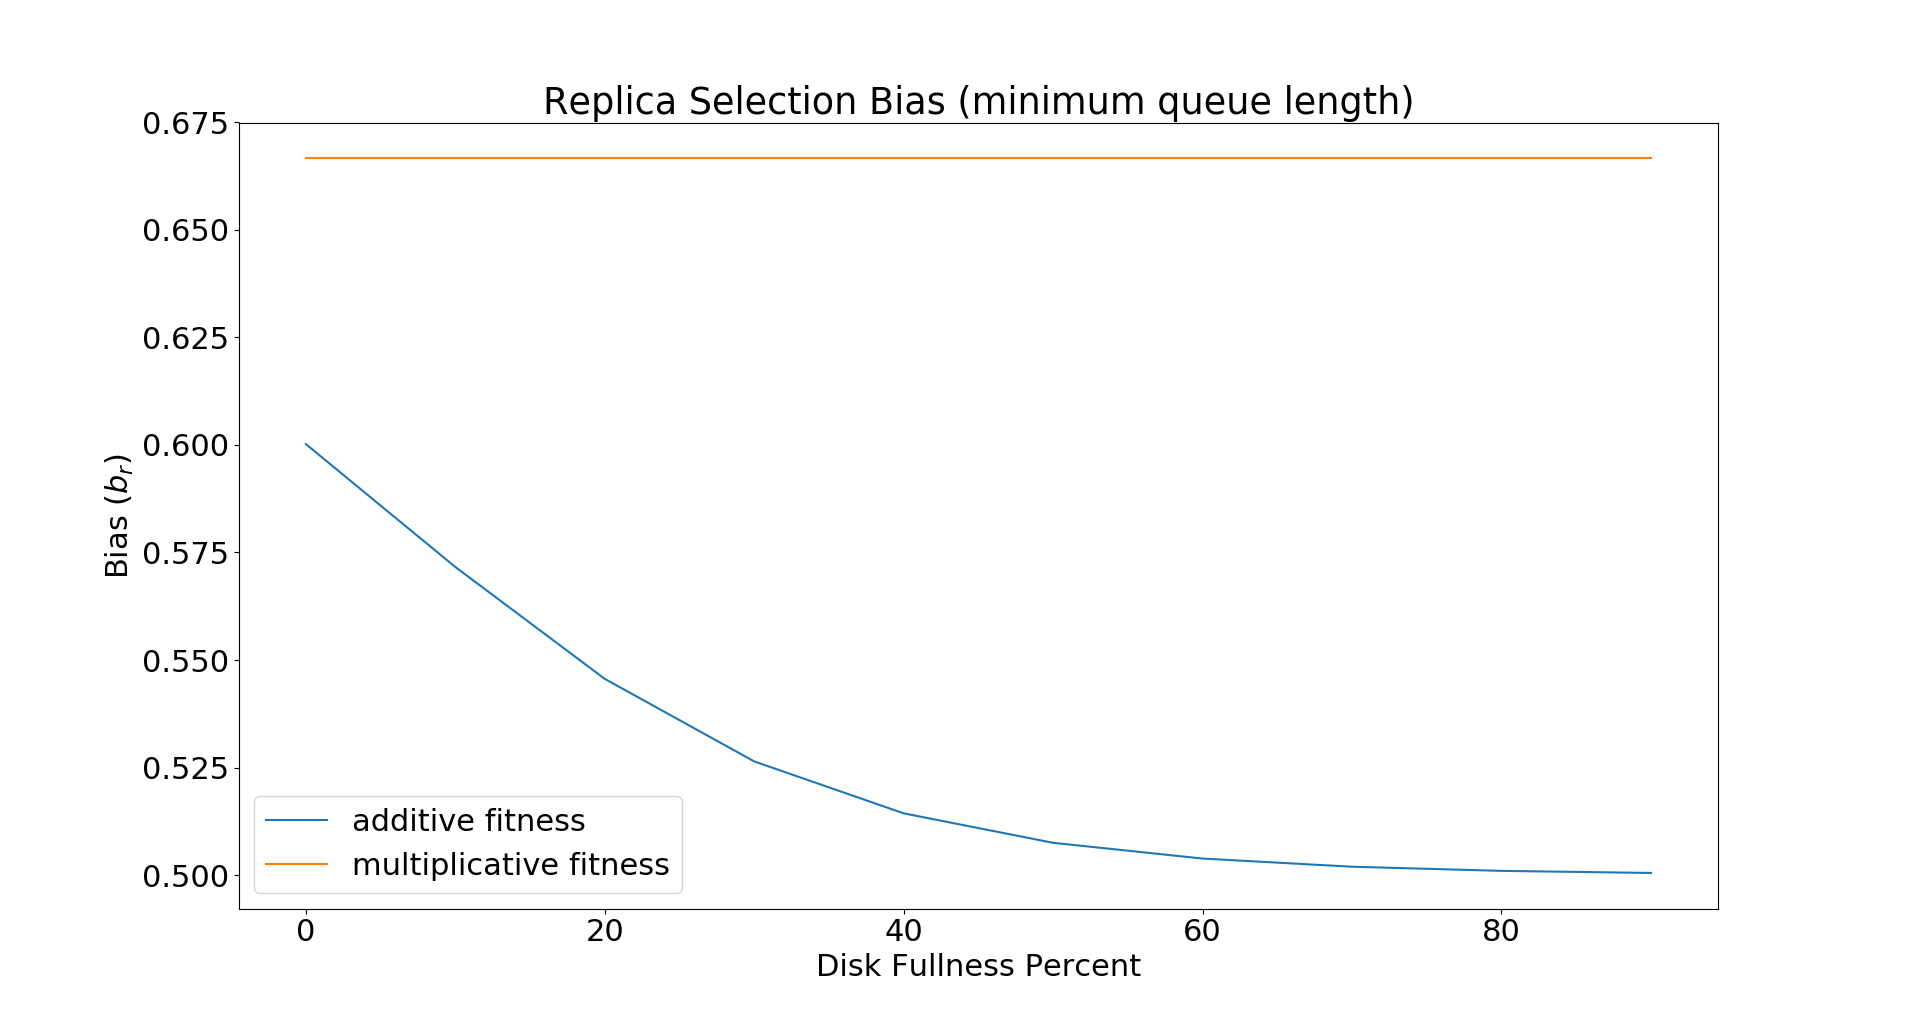
\includegraphics[scale=0.30]{images/replica_selection_bias_min_qlen.png} 
      \caption{$b_r$ values with static queue lengths at 1.}
      \label{fig:bias_min_qlen}
    \end{figure}

    We can see that for an additive fitness function, the bias towards a less
    utilized disk decreases as the disk fullness percentages for $d$ and $d'$
    increase, even though they still only differ by 10\% in the figure above.
    This is because the entire linear fitness function does not scale with each
    term, so we can conclude that the multiplicative fitness function is
    superior.

    \subsubsection{High Outstanding Operation Results}

    \begin{figure}[h]
      \centering
      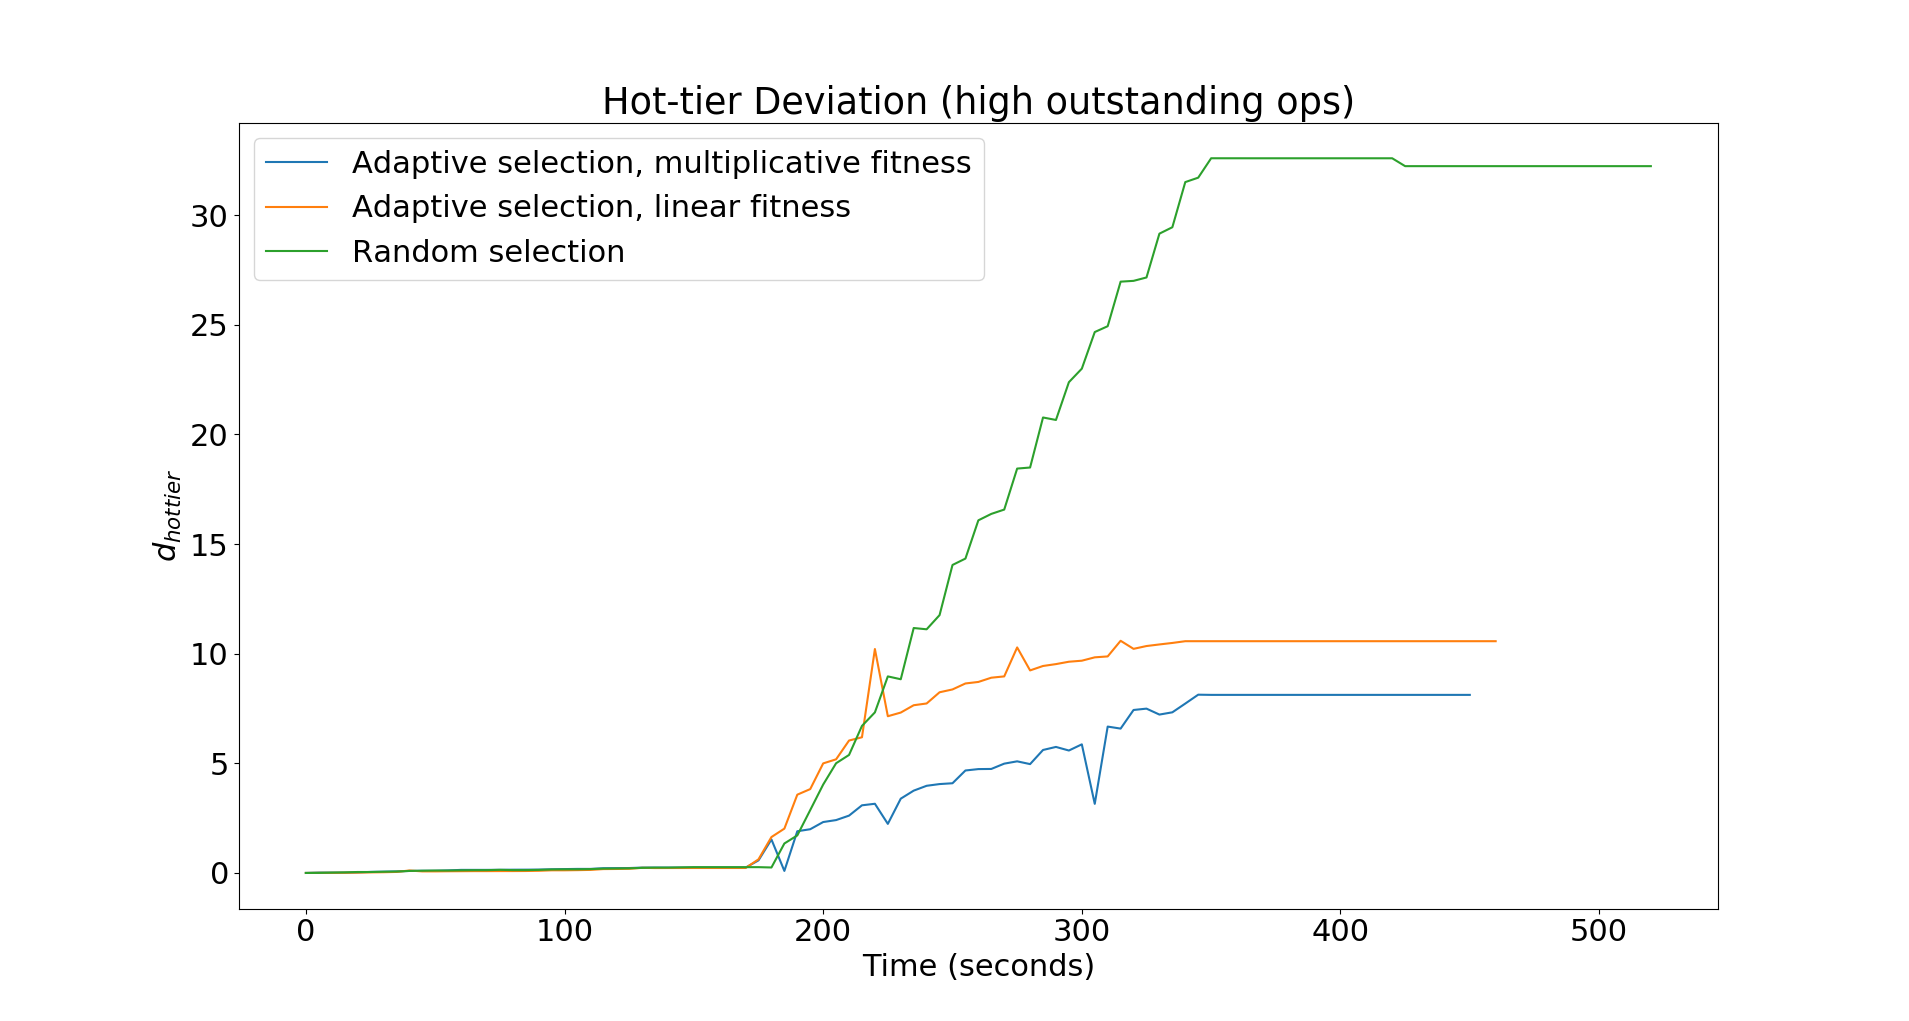
\includegraphics[scale=0.30]{images/high_outstanding_exp.png} 
      \caption{$d_{hot\ tier}$ values over time for low outstanding I/O
               operations.}
      \label{fig:high_outstanding_tier_disparity}
    \end{figure}


    In Figure \ref{fig:high_outstanding_tier_disparity}, we can see that both
    additive and multiplicative fitness functions reduce the disk fullness skew
    from 30\% to less than 10\%. Multiplicative fitness performs slightly
    better at minimizing $d_{hot\ tier}$ than additive fitness, possibly due to
    scaling the fitness value by the value of both the fullness and queue
    length terms, rather than weights.
  
  \subsection{Disk Queue Length Experiments}

  Since a low outstanding operation workload would not give useful
  information for measuring the effects of fitness-based replica selection on
  disk queue lengths, the high outstanding I/O operation experiment in the
  previous section was re-run for all fitness function types and for fitness
  function queue length term ceilings of 200 and 100. Figures
  \ref{fig:qlen_100} and \ref{fig:qlen_200} show a reduction in
  queue length quartiles when fitness-based selection is used for disks on
  nodes that host local workloads. Lower queue length ceilings are
  observed to provide better results in reducing the queue lengths for the
  worker nodes.

  \begin{figure}[!htb]
    \centering
    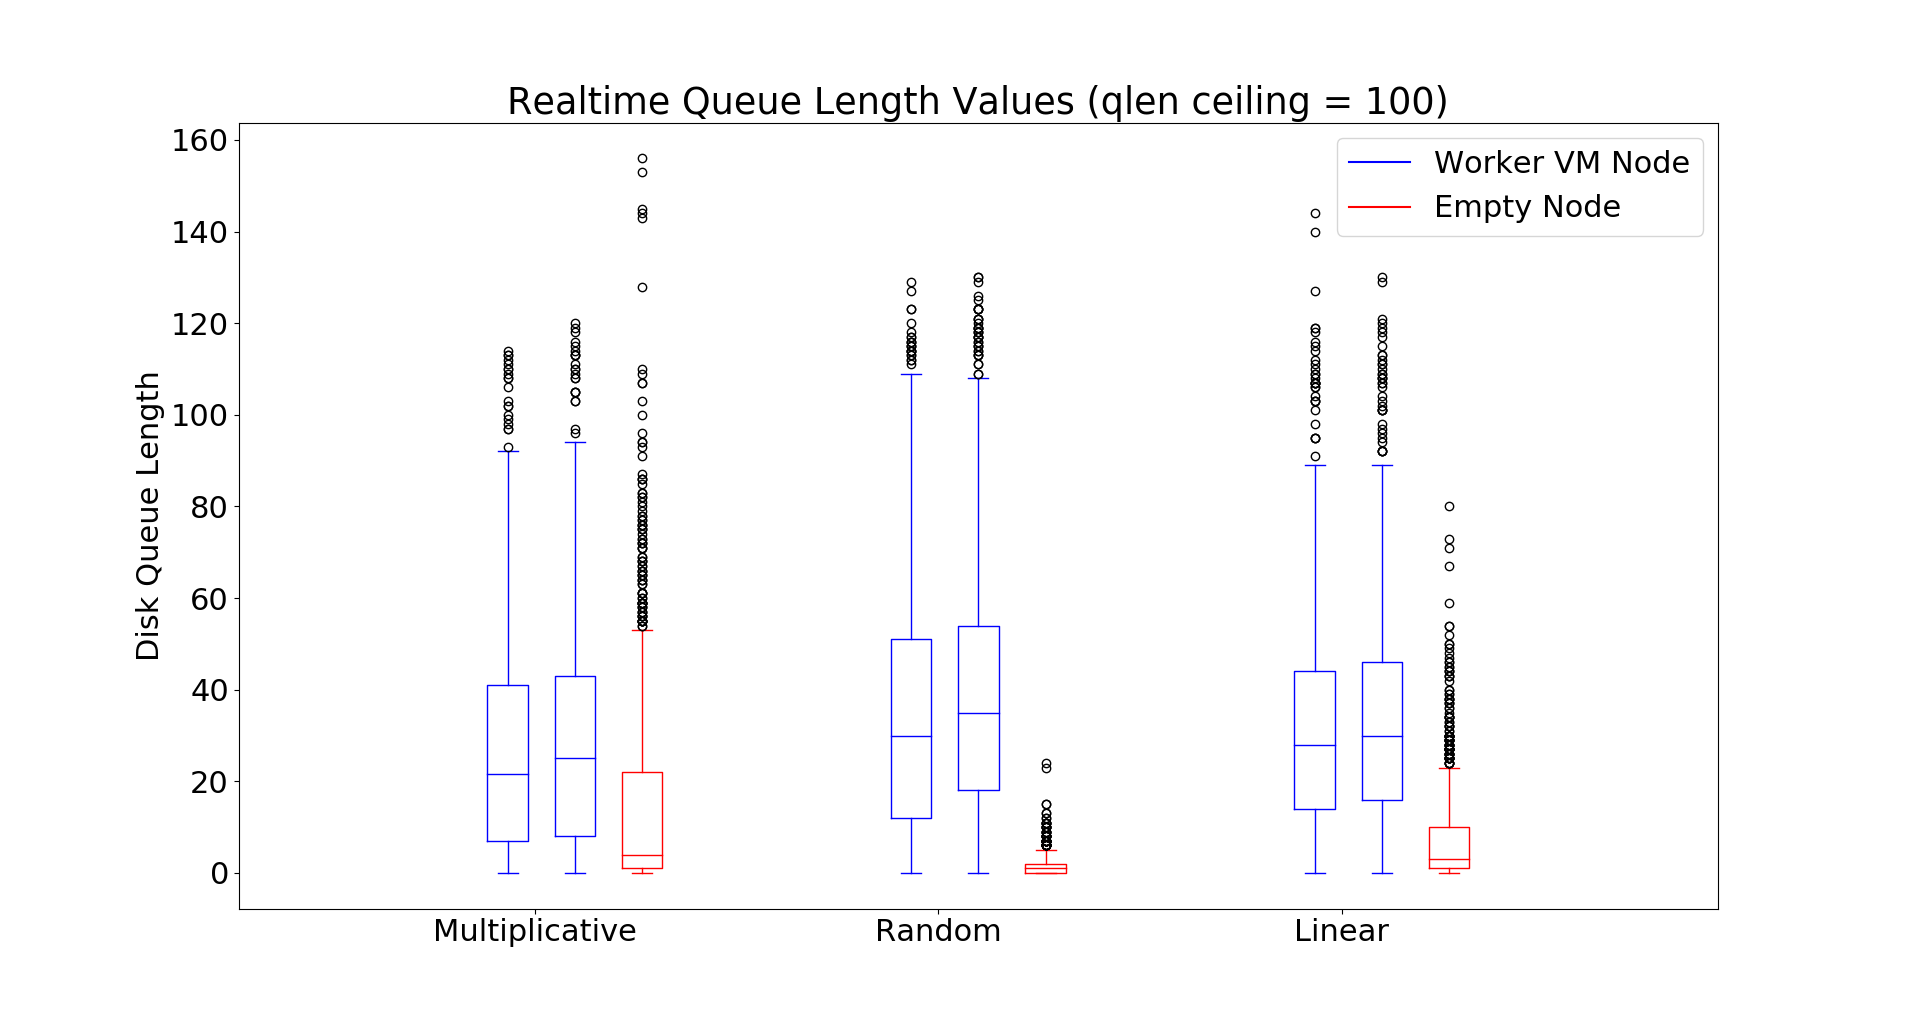
\includegraphics[scale=0.30]{images/qlen_100_box.png} 
    \caption{Queue lengths for all SSDs on the specified nodes sampled every 1
             second.}
    \label{fig:qlen_100}
  \end{figure}

  \begin{figure}[!htb]
    \centering
    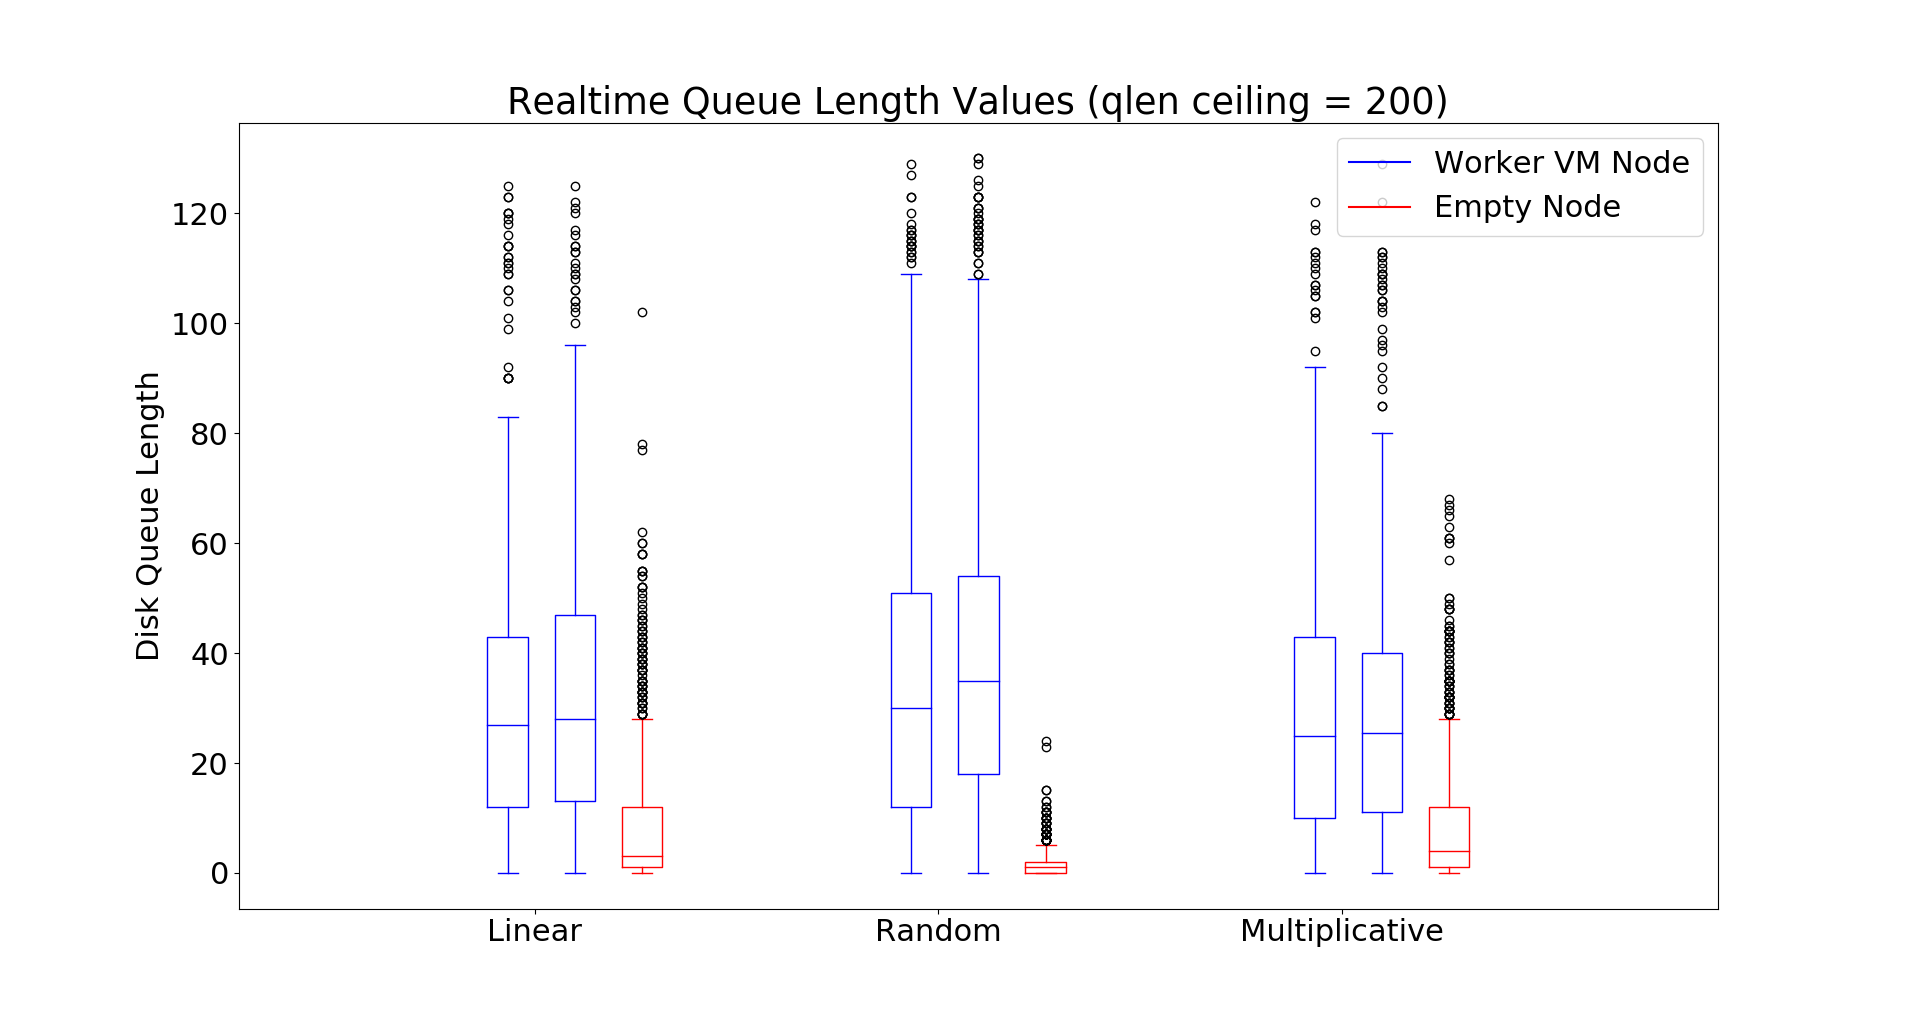
\includegraphics[scale=0.30]{images/qlen_200_box.png} 
    \caption{Queue lengths for all SSDs on the specified nodes sampled every 1
             second.}
    \label{fig:qlen_200}
  \end{figure}

%%%%%%%%%%%%%%%%%%%%%%%%%%%%%%%%%%%%%%%%%%%%%%%%%%%%%%%%%%%%%%%%%%%%%%%%%%%%%%%
\section{User Guide}

  \subsection{Scraping Data From the Nutanix Cluster}

  Stargate exposes a webserver on the CVM, listening on port 2009, that exposes
  various real-time stats such as the number of operations in flight, disk
  throughput, disk queue length, and many other pieces of information. I wrote
  a Python script to parse and derive the following information for each node:

  \begin{enumerate}
    \item SSD tier usage
    \item SSD tier availability
    \item SSD tier max capacity
    \item Read/Write counts for each disk
    \item Queue lengths for each disk
  \end{enumerate}

  The script will filter out all disks in the HDD tier and only pull the
  statistics for the SSD tier. Upon each invocation of the script, information
  is appended to a file for each node that is created if it is non-existent.
  The data is layed out in a CSV format for easy plotting via the Matplotlib
  library \cite{matplotlib}. For each experiment, the script was called every 5
  seconds via the command \verb|watch -n 5|.

  \subsection{Re-creating Experiments}

  An NX-1350 with VMware ESXi 5.5u2 hypervisor and a single 300GB SSD on each
  node was used for all experiments in this thesis. This means that for an RF2
  cluster, there is less than 150GB of useable hot tier available since a small
  amount of space is reserved on each disk for other services on the CVM.

  A single CentOS 6.5 worker VM was manually created on a single node with 4GB
  RAM, single 150GB disk, and installation of fio. The 150GB disk size ensures
  that the entire hot tier of each node will be fully utilized when the disk is
  filled via workload generation on each node. Each other node then clones the
  worker VM so that all nodes in the cluster have an identical VM and tier
  utilization.

  The fio script used to generate a sequential write workload on each node is
  as follows:
  
  \begin{verbatim}
    [global]
    direct=1
    ioengine=libaio
    bs=32k
    iodepth=128
    randrepeat=0
    group_reporting
    filesize=150G

    [job1]
    rw=write
    filename=/dev/sdb
    name=sequential-write
  \end{verbatim}

  The \verb|iodepth| variable is modified depending on the number of
  outstanding I/Os needed.

  When resetting the cluster for a new test, on the CVM I run
  \verb|cluster stop ; cluster destroy| and swap out the Stargate binary in
  the \verb|/home/nutanix/bin/| directory with the binary required for the next
  test. When ready, I recreate the Nutanix cluster via
  \verb|cluster -s <cvm IPs> create|. The process is then repeated for each
  test.

  \subsection{Plotting Data from Experiments}

  

%%%%%%%%%%%%%%%%%%%%%%%%%%%%%%%%%%%%%%%%%%%%%%%%%%%%%%%%%%%%%%%%%%%%%%%%%%%%%%%
\section{Future Work}

  \subsection{Real-time Fitness Feedback}

  The replica placement scheme shown in this work relies on periodic stats
  updates, so the system is always working with older stats for data placement
  decisions. One change that can be made to this system is to track the time to
  completion of various ops that place data on each disk and bias the replica
  placements towards the faster disks. This would require Stargate to keep
  historical latency data and would remove the dependence on a centralized
  stats repository.

  \subsection{Read Replica Selection}

  When choosing which replicas to read from, we always select local disks
  form the SSD tier and sometimes select remote HDDs at random. This process
  does not take the new disk fitness information that is available and would
  benefit from adapting read replica selection decisions based on the disk
  fitness values.

  \subsection{More Fitness Function Variables}

  The disk fitness values do not need to be limited to derivation from disk
  queue length and fullness percentage. The cluster tracks many other variables
  such as average node CPU utilization, number of Stargate failures in a
  specified time window, number of active user VMs, and data access patterns
  among other pieces of information. More investigation should occur to see how
  this data can be used to make better data placement decisions.

%%%%%%%%%%%%%%%%%%%%%%%%%%%%%%%%%%%%%%%%%%%%%%%%%%%%%%%%%%%%%%%%%%%%%%%%%%%%%%%
\section{Appendix}

  \subsection{Herding Behavior Due to Implementation Bug}

  During the 128 outstanding op experiments, herding behavior
  was observed unexpectedly after implementing fitness based replica placement
  as shown in Figure \ref{fig:herding_bug}. By default, disk usage and
  performance stats are supposed to be refreshed every 10 seconds. This is
  frequent enough to avoid herding behavior, but the 128 outstanding op
  experiments exhibited herding.

  \begin{figure}[h]
    \centering
    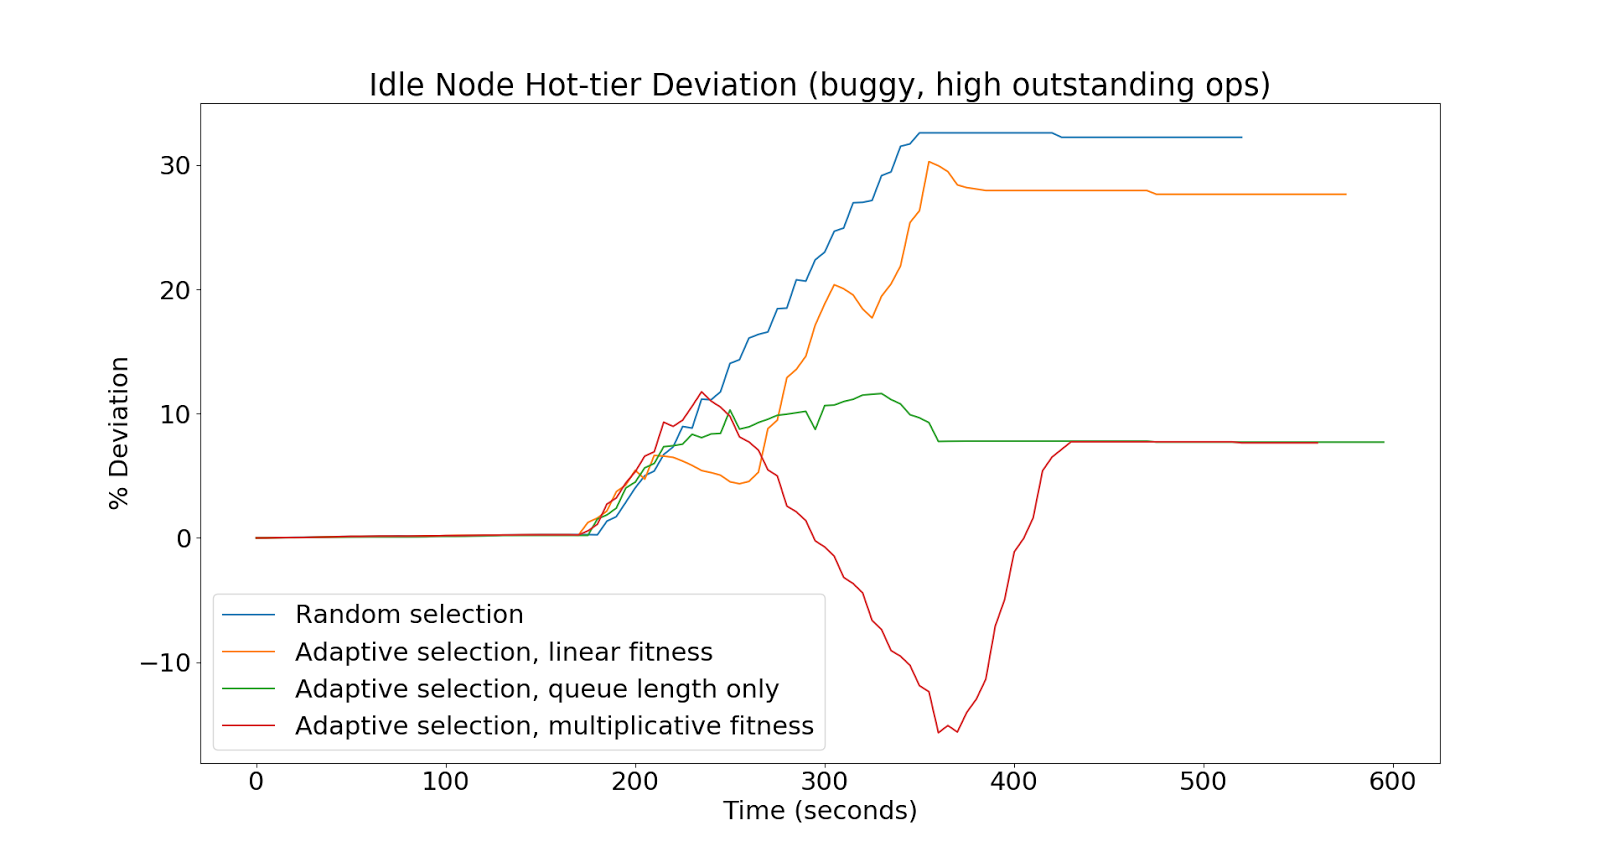
\includegraphics[scale=0.25]{images/buggy.png} 
    \caption{$d_{hot\ tier}$ values over time for low outstanding I/O
             operations. This set of experiments contains the stats update bug.}
    \label{fig:herding_bug}
  \end{figure}

  The experiment with additive fitness seemed to only exhibit mild herding
  behavior, whereas the test with multiplicative fitness showcased much more
  dramatic shifts in SSD usage skews. In conjunction with the complete absence
  of this behavior in the single outstanding op experiments, it was thought to
  be highly likely that this herding behavior was caused by a bug in the queue
  length term of the fitness functions. An additive fitness function is less
  affected by this bug due to the attenuated effect of each term in the fitness
  function.

  Within Stargate, we keep a mapping from disk ID to a DiskState object (called
  \verb|disk_map_|) containing information and cached statistics related to the
  disk. The disk performance and disk usage stats are two separate elements
  within the DiskState structure.

  Every 10 seconds, an alarm handler will execute and iterate through each
  active disk in the cluster and asynchronously query disk stats and bind a
  callback to each query to be executed when a response is received. Disk usage
  and performance lookups each have their own callback functions:

  \begin{center}
    \begin{tabular}{ | p{0.5\linewidth} | p{0.5\linewidth} | }
      \hline
      \textbf{Function Name} & \textbf{Description} \\ \hline
      \verb|UsageStatLookupCallback| & Decrement the outstanding stats lookup
                                       counter, acquire lock and populate
                                       performance stats in \verb|disk_map_|,
                                       and leave performance stats untouched.
                                       \\ \hline

      \verb|PerformanceStatLookupCallback| & Decrement outstanding stats
                                             lookup counter, lock and
                                             populate performance stats in
                                             \verb|disk_map_|, and leave
                                             usage stats untouched. \\ \hline

      \hline
    \end{tabular}
  \end{center}

  The two callbacks introduce a race condition regarding \verb|disk_map_| even
  though the structure is locked. Any time PerformanceStatLookupCallback
  returns before the callback for usage stats, all performance stats will be
  cleared and cause the fitness function to assume worst-case values for the
  queue length term.

  This problem was fixed by simply serializing our usage and performance stats
  lookups.

 \begin{thebibliography}{99}

   \bibitem{bible} Poitras, S. (n.d.) The Nutanix Bible. Retrieved August 09, 2017, from \url{http://www.nutanixbible.com/}

   \bibitem{cassandra} Lakshman, A., and Malik, P. (2008, August 25). Cassandra – A structured storage system on a P2P Network. Retrieved February 15, 2016, from \url{https://www.facebook.com/notes/facebook-engineering/cassandra-a-structured-storage-system-on-a-p2p-network/24413138919/}

   \bibitem{mapreduce} Dean, J., and Ghemawat, S. (2008). MapReduce: simplified data processing on large clusters. Communications of the ACM, 51(1), 107-113.

   \bibitem{hadoop} Hadoop, A. (2009). Hadoop. 2009-03-06].  \url{http://hadoop.apache.org}.

   \bibitem{xie2010} Xie, J., Yin, S., Ruan, X., Ding, Z., Tian, Y., Majors, J., ... and Qin, X. (2010, April). Improving mapreduce performance through data placement in heterogeneous hadoop clusters. In Parallel and Distributed Processing, Workshops and Phd Forum (IPDPSW), 2010 IEEE International Symposium on (pp. 1-9). IEEE.

   \bibitem{zaharia2008} Zaharia, M., Konwinski, A., Joseph, A. D., Katz, R.  H., and Stoica, I. (2008, December). Improving MapReduce Performance in Heterogeneous Environments. In OSDI (Vol. 8, No. 4, p. 7).

   \bibitem{adapt2012} Jin, H., Yang, X., Sun, X. H., and Raicu, I. (2012, June). Adapt: Availability-aware mapreduce data placement for non-dedicated distributed computing. In Distributed Computing Systems (ICDCS), 2012 IEEE 32nd International Conference on (pp. 516-525). IEEE.

   \bibitem{perez2003} Perez, J. M., Garcia, F., Carretero, J., Calderon, A., and Sanchez, L. M. (2003, May). Data allocation and load balancing for heterogeneous cluster storage systems. In Cluster Computing and the Grid, 2003. Proceedings. CCGrid 2003. 3rd IEEE/ACM International Symposium on (pp. 718-723). IEEE.

   \bibitem{breeder1993} Schlierkamp-Voosen, D., and Mühlenbein, H. (1993). Predictive models for the breeder genetic algorithm. Evolutionary Computation, 1(1), 25-49.

   \bibitem{baker1987} Baker, J. E. (1987, July). Reducing bias and inefficiency in the selection algorithm. In Proceedings of the second international conference on genetic algorithms (pp. 14-21).

   \bibitem{vitter1985} Vitter, J. S. (1985). Random sampling with a reservoir. ACM Transactions on Mathematical Software (TOMS), 11(1), 37-57.

   \bibitem{reservoir2006} Efraimidis, P. S., and Spirakis, P. G. (2006). Weighted random sampling with a reservoir. Information Processing Letters, 97(5), 181-185.

   \bibitem{chao1982} Chao, M. T. (1982). A general purpose unequal probability sampling plan.  Biometrika, 69(3), 653-656.

   \bibitem{esxi2008} Chaubal, C. (2008). The architecture of vmware esxi. VMware White Paper, 1(7).

   \bibitem{hdfs2008} Borthakur, D. (2008). HDFS architecture guide. HADOOP APACHE PROJECT http://hadoop. apache. org/common/docs/current/hdfs design. pdf, 39.

   \bibitem{suresh2015} Suresh, L., Canini, M., Schmid, S., and Feldmann, A. (2015). C3: Cutting tail latency in cloud data stores via adaptive replica selection. In 12th USENIX Symposium on Networked Systems Design and Implementation (NSDI 15) (pp. 513-527).

   \bibitem{hyperv2009} Velte, A., and Velte, T. (2009). Microsoft virtualization with Hyper-V. McGraw-Hill, Inc..

   \bibitem{paxos2005} Lamport, L. (2005). Generalized consensus and Paxos. Technical Report MSR-TR-2005-33, Microsoft Research.s

   \bibitem{azar1994} Y. Azar, A. Broder, A. Karlin, and E. Upfal. Balanced allocations. In Proceedings of the 26th ACM Symposium on the Theory of Computing, pages 593\{602, 1994.

   \bibitem{truncation1973} Crow, J. F., and Kimura, M. (1979). Efficiency of truncation selection. Proceedings of the National Academy of Sciences of the United States of America, 76(1), 396–399.

   \bibitem{2choice} Mitzenmacher, M. (2001). The power of two choices in randomized load balancing. IEEE Transactions on Parallel and Distributed Systems, 12(10), 1094-1104.

   \bibitem{matplotlib} Hunter, J. D. (2007). Matplotlib: A 2D graphics environment. Computing In Science and Engineering, 9(3), 90-95.

   \bibitem{python} Van Rossum, G., and Drake, F. L. (2003). Python language reference manual (p. 144). Network Theory.

   \bibitem{stl} Plauger, P. J., Lee, M., Musser, D., and Stepanov, A. A. (2000). C++ Standard Template Library. Prentice Hall PTR.

 \end{thebibliography}

\end{document}
